\documentclass[journal]{IEEEtran}

\usepackage{amssymb}
\setcounter{tocdepth}{3}
\usepackage{graphicx}

\usepackage{url}
\newcommand{\keywords}[1]{\par\addvspace\baselineskip
\noindent\keywordname\enspace\ignorespaces#1}

\usepackage[table]{xcolor}
\usepackage{tabularx}
\usepackage{qtree}
\usepackage{color, colortbl}
\usepackage{amsmath}
\usepackage{amssymb}
\usepackage{tikz}
\usepackage{pgfplots}
\usepackage{booktabs}
\usepackage{longtable}
\usepackage{supertabular}
\usepackage{caption}
\usepackage[hidelinks]{hyperref}
%\usepackage{IEEEtrantools}
%\usepackage{subfig}
\usepackage{float}
\usepackage{mathtools}
\usepackage{algorithm}
\usepackage{algorithmicx}
\usepackage{algpseudocode}
%\usepackage{commath}
\usepackage{physics}
\usepackage{algpseudocode}
\usepackage{authblk}
\usepackage{hyperref}
\usepackage{eqexpl}
\usepackage{makecell}
\usepackage{subcaption}
%\usepackage{subfigure}
\usepackage{multirow}
\usepackage{soul}
\usepackage{hhline}
\usepackage{stmaryrd}
\usepackage{import}
%\usepackage{filecontents}
\usepackage{catchfile}
%\usepackage{biblatex}
\usepackage[utf8]{inputenc}
\usepackage[english]{babel}
%\usepackage{natbib}
\usepackage{cite}
\usepackage{flexisym}
\usepackage{orcidlink}

\usepackage{coffeestains}




\DeclareMathOperator{\capacity}{Cap}
\DeclareMathOperator{\range}{range}
\DeclareMathOperator{\elems}{elems}
%\DeclareMathOperator{\range}{\mathfrak{R}}
\DeclareMathOperator{\HEncoder}{HEncoder}

\renewcommand{\algorithmicrequire}{\textbf{Input:}}
\renewcommand{\algorithmicensure}{\textbf{Output:}}


\pgfplotsset{compat=1.18}

\bibliographystyle{IEEEtran}








\begin{document}
	
	\title{
		Prediction-based Data Hiding of Multi-MSB Encrypted Images Using Huffman Coding in Cloud Services
	}
	
	\author{
		Li-Chiun Lin,	Cheng-Ta Huang and	 Shiuh-Jeng WANG*
		
		
		\thanks{Li-Chiun Lin and Shiuh-Jeng WANG* are with Information Cryptology Construction Lab, Department of Information Management, Central Police University, Taoyuan, Taiwan. Whom correspondence: Shiuh-Jeng WANG* \url{sjwang@mail.cpu.edu.tw}.}
		\thanks{Cheng-Ta Huang is with International Bachelor Program in informatics and Department of Information Management, Yuan Ze University, Taoyuan, Taiwan.}
	}
	
%	\institute{
%		$^1$ Information Cryptology Construction Lab, Department of Information Management, Central Police University, Taoyuan, Taiwan\\
%		$^2$ Internationa Bachelor Program in informatics, Yuan Ze University, Taoyuan, Taiwan \\
%		$^3$ Department of Information Management, Yuan Ze University, Taoyuan, Taiwan \\
%		$^\star$ Department of Information Management, Central Police University, Taoyuan, Taiwan\\
%		$^\star$ Whom correspondenc: \url{sjwang@mail.cpu.edu.tw}
%	}
	
	\maketitle
	%\coffeestainA{0.9}{0.85}{-25}{5cm}{1.3cm}
	
	\begin{abstract}
		The prosperity of cloud services stimulates the study of reversible data hiding in encrypted images, for which researchers dedicate to find better methods to adopt the new assumption that the ones who provide the cover images, a.k.a.\ the \emph{Content-owner}, are no longer the same as those who hide the secret message into them, a.k.a.\ the \emph{Data-hider}, and the \emph{Data-hider} might not always be allowed to know the actual content of cover image the \emph{Content-owner} provided, while the one who receives the stego image must be able to restore the exact cover image after extracting the secret.
		In this paper, an improved reversible data hiding in encrypted images algorithm is proposed and 
		our experimental results show that our proposal achieves better performance even in the worst-case scenario.
	\end{abstract}
	
	\begin{IEEEkeywords}
		Reversible data hiding, encrypted images, privacy protection, Huffman coding.
	\end{IEEEkeywords}
	
	\section{Introduction}
	\label{sec:intro}
	
	\IEEEPARstart{D}{ata}
	hiding is a technique used to prevent the conveyor from knowing the existence of a secret message while transporting it from the sender to the receiver. 
	While the cover image might inevitably suffer from distortion, a subset of the studies of data hiding is dedicated to meet the requirements that the cover image must be losslessly recovered after extracting the secret message, namely \emph{reversible data hiding} (RDH)~\cite{Coatrieux2009, Gao2009, Li2020}. 
	Furthermore, a subset within which even started to study the benefits of hiding secret messages into encrypted images, i.e., \emph{reversible data hiding in encrypted images} (RDHEI)~\cite{Zhang2011, Liu2020, Jain2021, Di2018}.
	The schemata are usually categorized into the following types. 
	
	In \emph{reserving room before encryption} (RRBE)~\cite{Ma2013, Agrawal2017, Liao2015}, as its name implies, a preprocessing procedure is applied to a cover image before applying an encryption procedure to it. 
	This type of schemata normally produces a \emph{label map} containing critical information for the following data hiding procedure. 
	This \emph{label map} is then considered as \emph{auxiliary information} and embedded into the cover image together with the secret message.
	
	In \emph{vacating room after encryption} (VRAE)~\cite{Puech2008, Wu2019, Li2018}, on the contrary, an encryption procedure is applied to a cover image before a post-process procedure can vacate some part of the encrypted cover image for a following data hiding procedure.
	
	Though the schemata of VRAE are more concise since the post-process and the data hiding process can be considered as one process, 
	those schemata of RRBE provides more capacity because they can exploit the similarity of adjacent pixels while the input of the post-process procedure of VRAE is an encrypted cover image, which is equivalent to random bytes in normal distribution.
	
	The schemata in the category of \emph{vacating room by encryption} (VRBE)~\cite{Liu2018, Yu2020} are more tricky since they adopt properties of certain cryptography algorithms to squeeze redundant space for data hiding while applying the encryption procedure, 
	but then they inevitably sacrifice the possibility to fully recover the cover image.
	
	When discussing RDHEI, a use case that comprises of three roles, namely the \emph{Content-owner}, the \emph{Data-hider} and the \emph{Receiver} is commonly adopted~\cite{Qin2015}.
	The \emph{Content-owner}, as its name suggested, is responsible for providing cover images, commonly analogies to a cloud service client user.
	The responsibility of the \emph{Data-hider} is to embed some secret message into the cover images, e.g., a cloud service provider might request to embed authentication data or annotations into the images. 
	The \emph{Receiver} could be the same as \emph{Data-hider} or any other entities that request the cover images and/or the embedded information.
	There are two extra requirements in this use case besides the fundamental goal of hiding the secret message. 
	\begin{enumerate}
		\item The \emph{Receiver} must receive the identical cover image as the \emph{Content-owner} provided.
		\item The \emph{Data-hider} must not know the content of the cover image.
	\end{enumerate}
	
	Researches in the field of RDHEI are hence raised to fulfill these two requirements.
%	Yin et al.\ proposed a method of RDHEI using adaptive multi-MSB prediction and Huffman coding~\cite{Yin2020}.
%	Their experimental results demonstrated the superiority of their method over the methods of~\cite{Puteaux2018, Chen2019, Puyang2019, Puteaux2019, Yi2019}.
	In this paper, we propose a new RDHEI method that achieve better embedding capacity than other state-of-the-art methods.

	The rest of the paper is organized as follows. 
	Related works are explained in Sec.\,\ref{sec:related}. Our proposal is described in Sec.\,\ref{sec:ours}. 
	Experimental results are demonstrated in Sec.\,\ref{sec:experimental}.
	Sec.\,\ref{sec:conclusion} concludes this paper. 


	\section{Related Work}
	\label{sec:related}
	
%	\subsection{MSB-Prediction Based Method}

	Puteaux et~al.\ proposed a MSB-prediction based RDHEI method~\cite{Puteaux2018}, which exploited the interesting fact that neighboring pixels will very likely to have same MSB values, thus can be used for data hiding. 
	Yi et~al.\ proposed a RDHEI method which uses parametric binary tree labeling technique to harvest the benefit of pixel correlation in small image blocks~\cite{Yi2019}.
	Chen et~al.’s method adopted extended run-length coding on bit planes to vacate room for embedding~\cite{Chen2019}.
	Yin et~al.\ proposed a RDHEI method base on median edge detector (MED) predictor
	%r~\cite{Weinberger2000} 
	and Huffman coding technique~\cite{Yin2020}.
	%~\cite{IRE1952}
	Their method complied with the common use case that consists of the \emph{Content-owner}, the \emph{Data-hider} and the \emph{Receiver}.
%	The responsibilities of each role are defined in Fig.\,\ref{fig:yin_framework}. 
	Their method consists of the following steps. 
	\begin{enumerate}
		\item The \emph{Content-owner} generate \emph{label map} from the cover image using MED predictor.
		\item The \emph{Content-owner} encrypts the cover image using key \(K_e\).
		\item The \emph{Content-owner} encodes \emph{label map} using a predefined Huffman coding tree.
		\item The \emph{Content-owner} embeds the encoded \emph{label map} into the encrypted cover image using multi-MSB substitution.
		\item The \emph{Data-hider} extracts and decodes the \emph{label map} from the encrypted cover image. 
		\item The \emph{Data-hider} encrypts secret message using key \(K_d\).
		\item The \emph{Data-hider} uses the \emph{label map} and the same predefined Huffman coding tree to encode the secret message.
		\item The \emph{Data-hider} embeds the encoded \emph{label map} and secret message into the encrypted cover image using multi-MSB substitution.
		\item The \emph{Receiver} extracts and decodes the \emph{label map} from the encrypted cover image.
		\item The \emph{Receiver} can extract and decrypt the secret message if the \emph{Receiver} possesses key \(K_d\).
		\item The \emph{Receiver} can restore and decrypt the cover image if the \emph{Receiver} possesses key \(K_e\).
	\end{enumerate}

	
	\section{Proposed Method}
	\label{sec:ours}
	
	\begin{figure*}[!t]
		\centering
		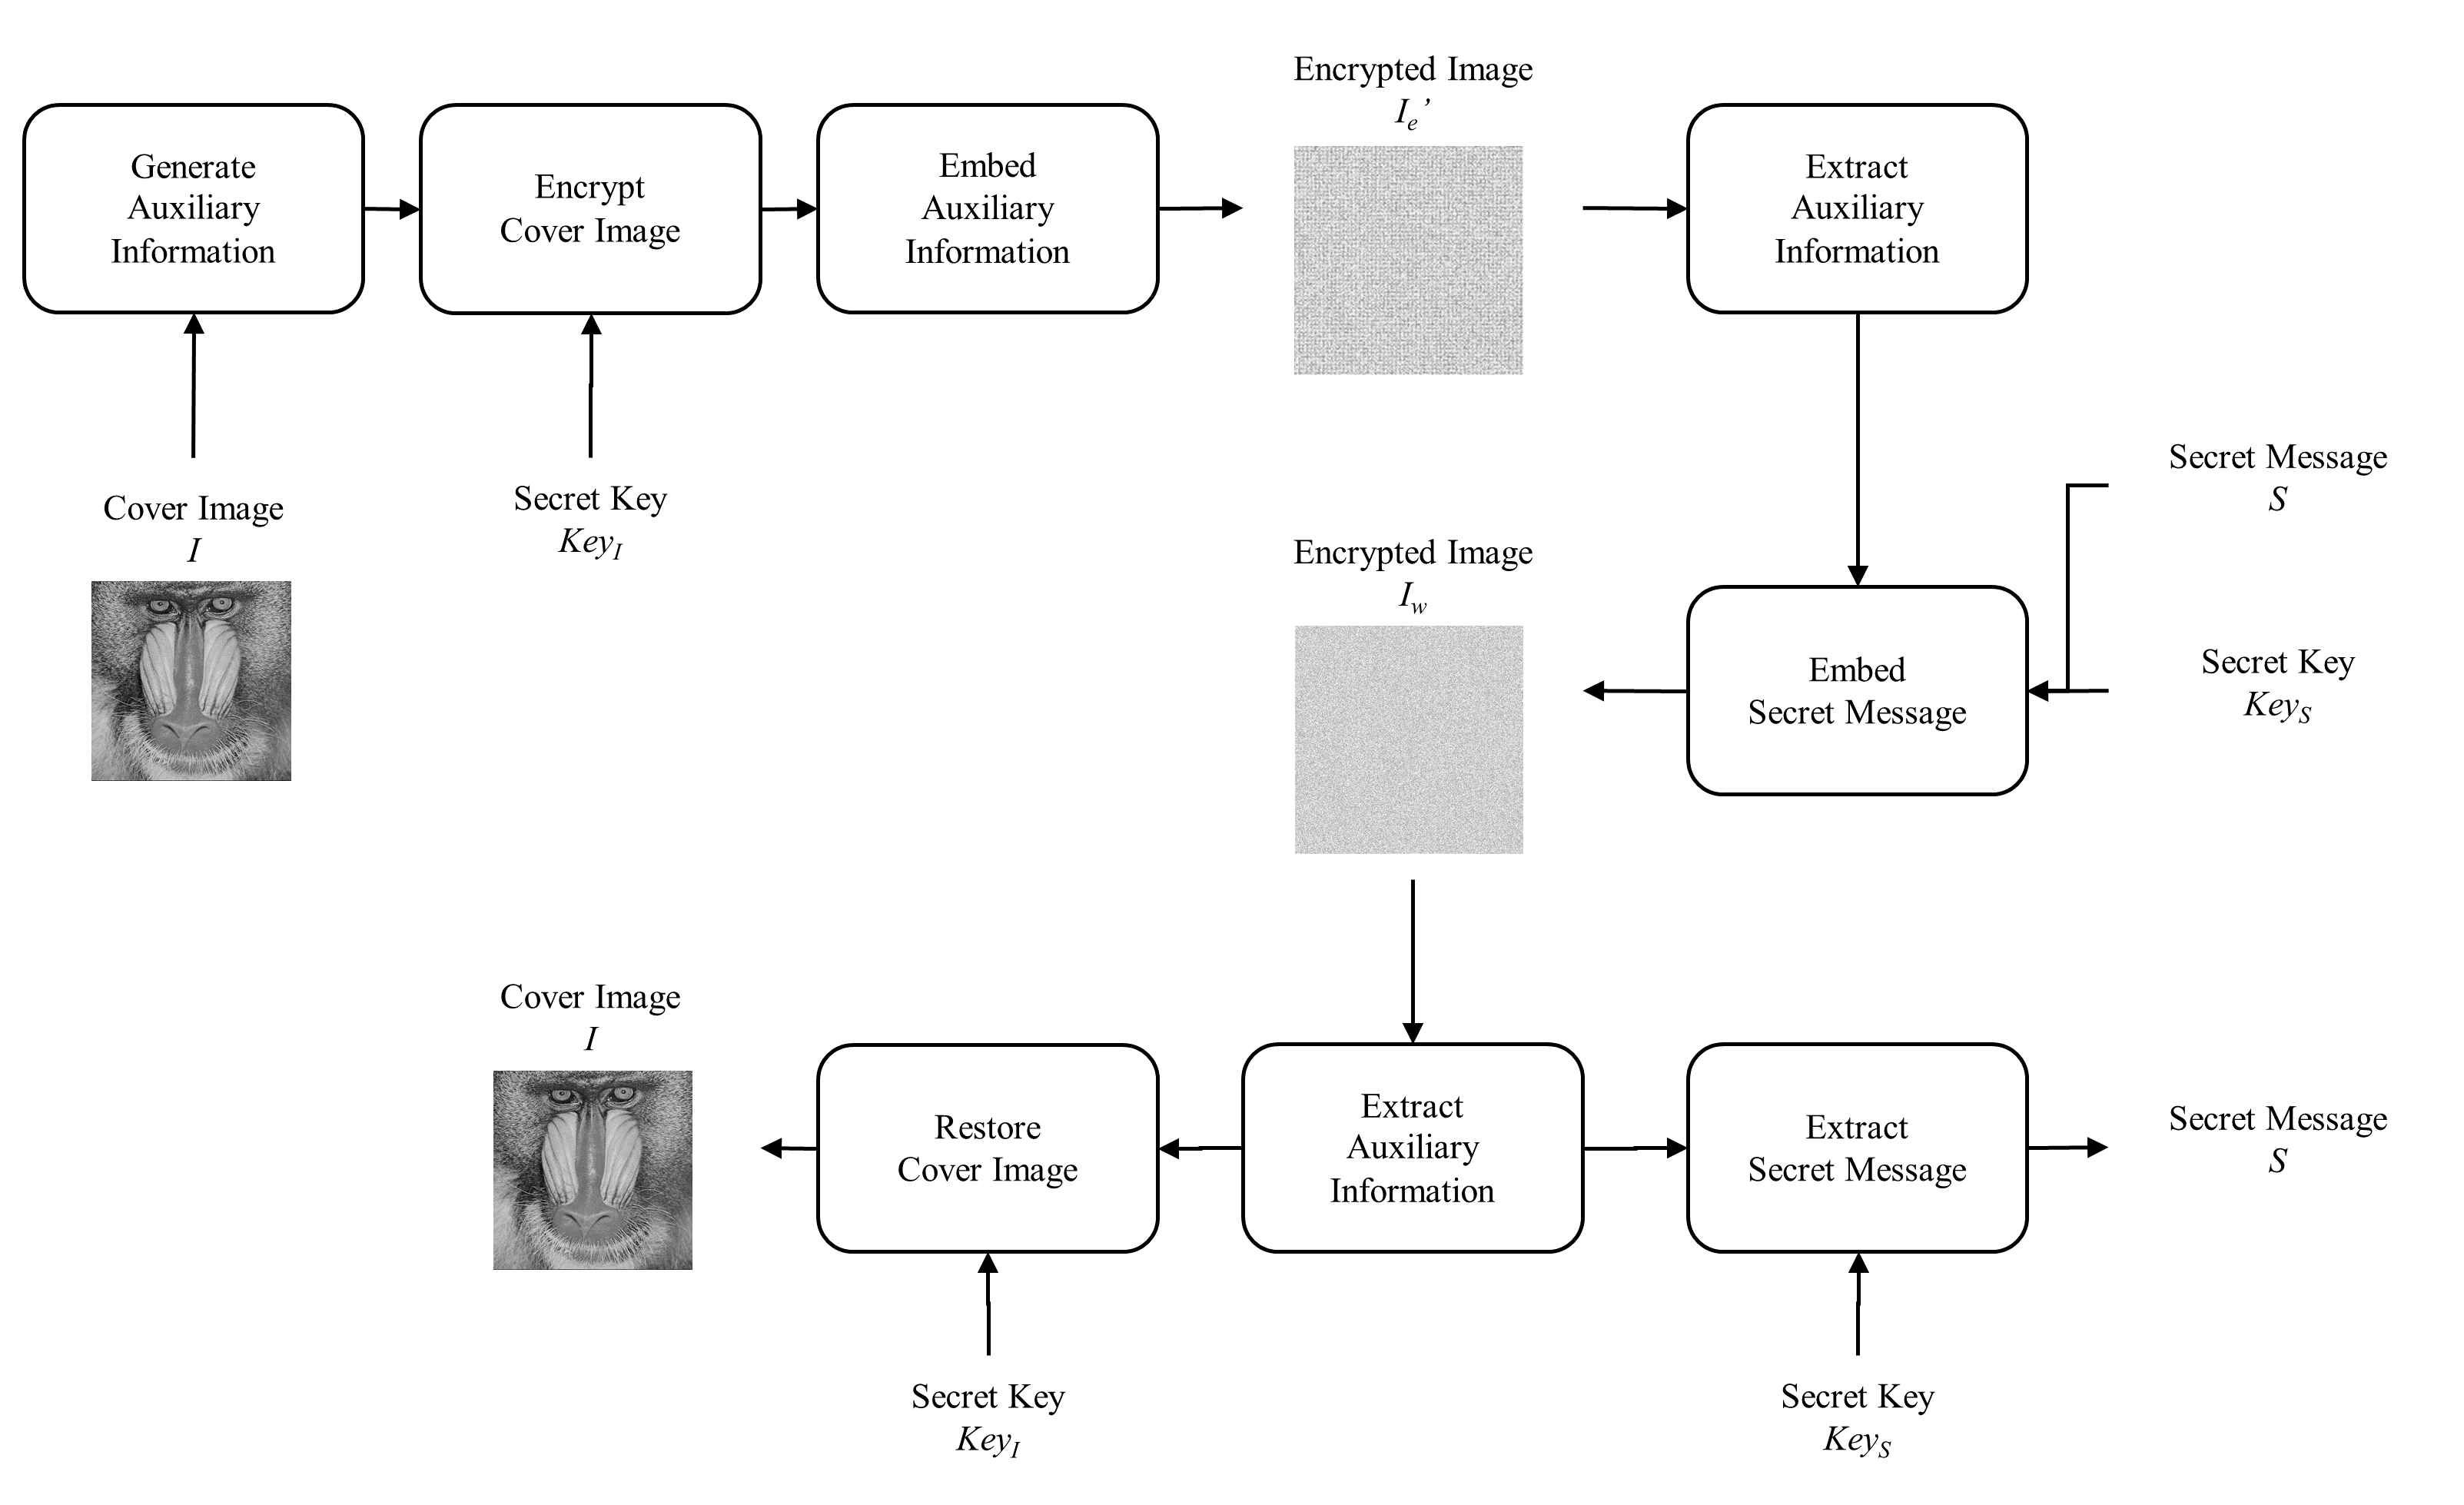
\includegraphics[width=\linewidth]{img/flow-chart}%
		\caption{Flow chart of the proposed method.}
		\label{fig:flowchart}
	\end{figure*}
	
	In this section, we propose a new RDHEI method base on the same use case as~\cite{Yin2020}. 
	Our proposal adopts the same flow char as Fig.\,\ref{fig:flowchart}. 
	Our method is reversible, achieves higher embedding capacity and comply with the typical requirements described in Sec.\,\ref{sec:intro}. 
	
	\subsection{Generate Auxiliary Information}
	
	\begin{figure}[!t]
		\centering
		\begin{tabular}{|c|c|c|c|c|} 
			
			\multicolumn{1}{c}{\phantom{\(x_{i-1, j-1}\)}} & \multicolumn{1}{c}{\phantom{\(x_{i-1, j-1}\)}} &
			\multicolumn{1}{c}{\phantom{\(x_{i-1, j-1}\)}} & \multicolumn{1}{c}{\phantom{\(x_{i-1, j-1}\)}} & \multicolumn{1}{c}{\phantom{\(x_{i-1, j-1}\)}}  
			\\
			\hline
			\(x_{0, 0}\) & \(x_{0, 1}\) & \(x_{0, 2}\)      & \(\dots\)    & \(x_{0, w}\) \\ \hline
			\(x_{1, 0}\) & \(\dots\)    & \(\dots\)         & \(\dots\)    & \(\dots\)    \\ \hline 
			\(x_{2, 0}\) & \(\dots\)    & 
			\cellcolor{black!10} \(x_{i-1, j-1}\) & \cellcolor{black!10}\(x_{i - 1, j}\) & \(\dots\)   \\ \hline 
			\(\dots\)    & \(\dots\)    & 
			\cellcolor{black!10}\(x_{i, j - 1}\)  & \cellcolor{black!20}\(x_{i, j}\)     & \(\dots\)    \\ \hline 
			\(x_{h, 0}\) & \(\dots\)    & \(\dots\)          & \(\dots\)        & \(x_{h, w}\) \\ \hline 
			
			\multicolumn{5}{c}{{}}\\
			
			\hline
			\rowcolor{black!30}
			\cellcolor{black!30}\(N/A\)   & \(N/A\)       &\(N/A\)      & \(\dots\)                       &\(N/A\)      \\ \hline
			\cellcolor{black!30}\(N/A\)   & \(pv_{1, 1}\) & \(pv_{1, 2}\) & \(\dots\)                        & \(pv_{1, w}\) \\ \hline
			\cellcolor{black!30}\(N/A\)   & \(pv_{2, 1}\) & \(\dots\)     & \(\dots\)                        & \(\dots\)    \\ \hline 
			\cellcolor{black!30}\(\dots\) & \(\dots\)     & \(\dots\)     & \(\dots\)                         & \(\dots\)    \\ \hline 
			\cellcolor{black!30}\(\dots\) & \(\dots\)    & \(\dots\)     & \cellcolor{black!20}\(pv_{i, j}\) & \(\dots\)    \\ \hline 
			\cellcolor{black!30}\(N/A\)   & \(pv_{h, 1}\) & \(\dots\)    & \(\dots\)                        & \(pv_{h, w}\) \\ \hline 
		\end{tabular}
		
		\caption{The MED predictor.}
		\label{fig:xpv}
	\end{figure}

	\begin{align}
		\label{eq:pv}
		pv_{i, j} & = 
		\begin{cases}
			\text{undefined}							   , \quad \text{if } i = 0 \vee j = 0, \\
			\max(x_{i - 1, j}, x_{i, j - 1})               , \\
			\quad \text{if } x_{i - 1, j - 1} \leq \min(x_{i - 1, j}, x_{i, j - 1}), \\
			\min(x_{i - 1, j}, x_{i, j - 1})               , \\
			\quad \text{if } x_{i - 1, j - 1} \geq \max(x_{i - 1, j}, x_{i, j - 1}), \\
			x_{i - 1, j} + x_{i, j - 1} - x_{i - 1, j - 1} , \quad \text{otherwise}. 
		\end{cases} \\
		%
		%		\label{eq:pe}
		%		pe_{i, j} & = 
		%		\begin{cases}
			%			\text{undefined}, &\text{if } i = 0 \vee j = 0, \\
			%			pv_{i, j} \oplus x_{i, j} , & \text{otherwise}.\\
			%		\end{cases} \\
		\label{eq:pe2}
		pe_{i, j} &= 
		\begin{cases}
			\text{undefined},             & \text{if } i = 0 \wedge  0 \leq j < REF ,\\
			x_{i, j - 1} \oplus x_{i, j}, & \text{if } i = 0 ,\\
			x_{i - 1, j} \oplus x_{i, j}, & \text{if } j = 0 ,\\
			pv_{i, j} \oplus x_{i, j}, 	  & \text{otherwise}.
		\end{cases} \\
		%
		\label{eq:t}
		t_{i, j} &= 
		\begin{cases}
			\text{undefined},             & \text{if } i = 0 \wedge  0 \leq j < REF ,\\
			8,&  \text{if } pe_{i, j} = 0,       \\
			7 - \lfloor \log_2(pe_{i, j}) \rfloor ,&  \text{if } pe_{i, j} \neq  0.
		\end{cases} 	
	\end{align}
	
	For all pixel \(x_{i, j} \) in a cover image \(I\), the predicted value \(pv_{i, j}\) of MED predictor is defined as~\eqref{eq:pv} and illustrated in Fig.\,\ref{fig:xpv}.
	The predicted error \(pe_{i, j}\) between each pixel and its predicted value is defined as~\eqref{eq:pe2}.
	Each \(pe_{i, j}\) has a corresponding value \(t_{i, j}\), as defined in~\eqref{eq:t}, represents the embedding capacity the corresponding pixel \(x_{i, j}\) can provide.
	

	Let \(\mathbf{T}\) be a matrix containing all \(t_{i, j}\), \(1 \leq i < h, 1\leq j < w\), where \(h\) and \(w\) denote the height and the width of \(I\), respectively.
	
	Let \(\mathbf{F}\) be the frequency table of \(\mathbf{T}\).
%	\begin{equation}
%		\label{eq:f}
%		\mathbf{F} = (f_0, \dots, f_8),  \text{where } f_v = \# \{ v \in \mathbf{T} \}.
%	\end{equation}
	
%	Let \(\mathbf{V}\) be a monotonically increasing vector consisting of all possible values in \(\mathbf{T}\) sorted by its frequency in \(\mathbf{F}\).
%	\begin{multline}
%		\label{eq:v}
%		\mathbf{V} = (v_0, \dots, v_8), \\
%		\text{where } \forall v_i, v_j \in \mathbf{V} \colon i \leq j \iff f_{v_i} \leq f_{v_j} .
%	\end{multline}
	
	Let \(\mathrm{cap}(t)\) be a function defined for all \(t \in \mathbf{T}\).
%	, representing the capacity each \(t_{i, j} = v\) can provide.
	\begin{equation}
		\label{eq:cap}
		\mathrm{cap}(t) = 
		\begin{cases}
			8     ,&  \text{if } t = 8,       \\
			t + 1 ,&  \text{if } 0 \leq t \leq 7.
		\end{cases} 
	\end{equation}
	
%	\subsection{Build Huffman coding tree}
	\label{sec:improvetree}
	Apply the Huffman tree building algorithm (as shown in Algorithm~\ref{algo:buildtree}) on \(\mathbf{F}\).
	
%	We observed that Yin et al.\ introduced their method based on a predefined Huffman tree as shown in Fig.\,\ref{fig:fixtree} 
%	without clarifying the pros and cons behind this design decision. 
%	We found that this fixed predefined tree topology constrains the true ability of Huffman coding. 
%	When we apply the standard Huffman coding algorithm, as shown in Algorithm~\ref{algo:buildtree}, its full power can be released~\cite{IRE1952, Leeuwen2008a}.
	
	\begin{figure}[!t]
		\begin{algorithm}[H]
		\caption{Build a Huffman coding tree.}
		\label{algo:buildtree}
		
		\begin{algorithmic}[1]
			\Require the frequency table \(\mathbf{F}\).
			\Ensure a Huffman coding tree \(\mathbf{H}\).
			
			\State \(nodes \gets \emptyset\)
			\ForAll{\(f_v \in \mathbf{F}\)}
			\State Create a node \(n\) with frequency \(f_v\) and value \(v\).
			\State \(nodes \gets nodes \cup \{n\}\).
			\EndFor
			
			\While{\(\vert nodes \vert \; > 1\)}
			\State Find \(n1 \in nodes\) with the least \(f_1\).
			\State \(nodes \gets nodes \setminus \{n1\}\).
			
			\State Find \(n2 \in nodes\) with the least \(f_2\).
			\State \(nodes \gets nodes \setminus \{n2\}\).
			
			\State Create a node \(n3\) with 
			\State\hspace{\algorithmicindent} \(f \leftarrow f_1 + f_2\)
			\State\hspace{\algorithmicindent} \(left \leftarrow n1\).
			\State\hspace{\algorithmicindent} \(right \leftarrow n2\).
			
			\State \(nodes \gets nodes \cup \{n3\}\).
			\EndWhile
		\end{algorithmic}
	\end{algorithm}
	\end{figure}

	Let \(\mathrm{encode}(t)\) be the Huffman encoding of \(t \in \mathbf{T}\) using \(\mathbf{H}\), and \(\mathrm{decode}(h)\) be its inverse. 
%	\begin{align}
%		\label{eq:encode}
%		&\mathrm{encode}(t) = c,
%		\\
%		\label{eq:decode}
%		&\mathrm{decode}(c) = t ,
%		\\
%		&\quad \text{where } \exists i \in [0, 8] : v_i \in \mathbf{V} \wedge h_i \in \mathbf{H} \wedge v_i = t \wedge h_i = c. \notag
%	\end{align}

	Define \(\mathrm{payload}(t)\) as the differences between the capacity of $t$ and the length of its Huffman encoding. 
	\begin{equation}
		\label{eq:payload}
		\mathrm{payload}(t) = \mathrm{cap}(t) - \vert \mathrm{encode}(t) \vert .
	\end{equation}
	
	Let \(\mathbf{T^\prime}\) be the concatenation of Huffman code of \(\mathbf{T}\).
%	 and \(LEN\) be its length.
	\begin{align}
		\label{eq:encodeT1}
		\mathbf{T^\prime} &= \bigparallel_{i = 1}^h  { \bigparallel_{j = 1}^w \mathrm{encode}(t_{i, j})}. %\\
%		\label{eq:countlen}
%		LEN  &= \sum_{v \in \mathbf{V}} (f_v \times \lvert \mathrm{encode}(v) \rvert).
	\end{align}

	\begin{figure}[!t]
		\tiny
		\Tree[ 
		[.0 [.0 \{00\}\\5 ]
		[.1 [.0 \{010\}\\7 ] [.1 \{011\}\\8 ]]]
		[.1 [.0 [.0 \{100\}\\3 ]
		[.1 [.0 \{1010\}\\2 ]
		[.1 [.0 \{10110\}\\1 ] [.1 \{10111\}\\0 ]]]]
		[.1 [.0 \{110\}\\6 ] [.1 \{111\}\\4 ]]]] 
		\caption{The Huffman tree of \emph{Lena} \(512 \times 512\).}
		\label{fig:lenatree}
	\end{figure}

	\begin{table}
		\centering
		\caption{Huffman coding of \emph{Lena} \(512 \times 512\).}
		\begin{tabular}{c@{\;}rl@{}c@{\;}c@{\;}c@{}r}
			\toprule  
			\(t\) &   \multicolumn{1}{c}{\(f_t\)} &     \multicolumn{1}{c}{\(\mathrm{encode}(t)\)}  &  \(\mathrm{cap}(t)\) &    \(\vert \mathrm{encode}(t) \vert\)    & \(\mathrm{payload}(t)\)  & \(\Delta\) \\
			\midrule  
			$0$ & $9866$  & $10111$ & $1$ & $5$ & $-4$ & $-39464$ \\ 
			$1$ & $9751$  & $10110$ & $2$ & $5$ & $-3$ & $-29253$ \\ 
			$2$ & $15315$  & $1010$ & $3$ & $4$ & $-1$ & $-15315$ \\ 
			$3$ & $33301$  & $100$ & $4$ & $3$ & $+1$ & $+33301$ \\ 
			$4$ & $44672$  & $111$ & $5$ & $3$ & $+2$ & $+89344$ \\ 
			$5$ & $53588$  & $00$ & $6$ & $2$ & $+4$ & $+214352$ \\ 
			$6$ & $41932$  & $110$ & $7$ & $3$ & $+4$ & $+167728$ \\ 
			$7$ & $24451$  & $010$ & $8$ & $3$ & $+5$ & $+122255$ \\ 
			$8$ & $29198$  & $011$ & $8$ & $3$ & $+5$ & $+145990$ \\ 
			\midrule 
			$\sum$ & $262074$   && $1476121$ & $787183$ &    $+688938$ & \\ 
			\bottomrule   
		\end{tabular}
		\label{tab:shrlena}
	\end{table}
	
	As an example, the tree topology of applying Algorithm~\ref{algo:buildtree} to \emph{Lena} \(512 \times 512\) is shown in Fig.\,\ref{fig:lenatree} and the statistic data is given in Table~\ref{tab:shrlena}. 
%	The Huffman encoding result is given in Table~\ref{tab:msblena}.
	
	The columns are in conformity with their definitions and the column \emph{\(\Delta\)} represents the result of \(f_t \times \mathrm{payload}(t)\). 
	Each cell in the row \emph{\(\sum\)} represents the weighted summation of the corresponding column.
	
	\begin{figure}[!t]
		\begin{algorithm}[H]
			\caption{Tree Serialization.}
			\label{algo:serial}
			
			\begin{algorithmic}[1]
				\Require Huffman tree \(\mathbf{H}\).
%				\Require size \(s\) of bits of each value \(v\).
				\Ensure  bit sequence \(topology\).
				\Ensure  bit sequence \(value\).
				
				\State \(topology \gets \emptyset\).
				\State \(value    \gets \emptyset\).
				
				\State \Call{SerializeTree}{$\mathbf{H}$}.
				\\
				
				\Procedure{SerializeTree}{$node$}   
				\If{\(node\) is a leaf}
				\State 		Let leaf value \(v\) be presented as \(v_0 \Vert \cdots \Vert v_3\).
				\State 		\(topology \gets topology \Vert 0\).
				\State 		\(value \gets value \Vert v_0 \Vert \cdots \Vert v_3\).
				\Else
				\State		 \(topology \gets topology \Vert 1\).
				\State 		\Call{SerializeTree}{$node.left$}.
				\State 		\Call{SerializeTree}{$node.right$}.
				\EndIf
				\EndProcedure
			\end{algorithmic}
		\end{algorithm}
	\end{figure}
	
	\begin{figure}[!t]
		\begin{algorithm}[H]
			\caption{Tree Deserialization.}
			\label{algo:unserial}
			
			\begin{algorithmic}[1]
				\Require bit sequence \(topology\).
				\Require bit sequence \(value\).
%				\Require size \(s\) of bits of each value \(v\).
				\Ensure Huffman tree \(\mathbf{H}\).
				
				\State \Call{UnserializeTree}{$topology, value$}.
				\\
				\Function{UnserializeTree}{$topology, value$}   
				\State Read 1 bit \(b\) from \(topology\).
				\If{\(b = 0\)}
				\State 		Read \(4\) bits from \(value\).
				\State 		Create a node \(n\) with \(v = (value_0, \dots, value_3)\).
				\Else
				\State 		Create a node \(n\) with
				\State \(left \gets\) \Call{UnserializeTree}{$topology, value$} 
				\State \(right \gets\) \Call{UnserializeTree}{$topology, value$}.
				\EndIf
				\State \Return \(n\).
				\EndFunction
			\end{algorithmic}
		\end{algorithm}
	\end{figure}
	
	Tree serialization follows Algorithm~\ref{algo:serial}. The reverse process follows Algorithm~\ref{algo:unserial}.
	In Algorithm~\ref{algo:serial}, a Huffman tree of \(9\) leaves has \(2 \times 9 -1 = 17\) nodes, each needs one bit to represent its role, where \(1\) indicates an internal node and \(0\) indicates a leaf~\cite{Pu2006}. 
	Each leaf has a value \(0 \leq v \leq 8\), thus four bits are enough to store each leaf value, i.e., \(4 \times 9 = 36\) bits. 
	Hence we needs \(53\) bits to serialize the tree topology and leaf values.
	
	
	
	
	\subsection{Encrypt Cover Image}
	
	The cover image \(I\) is encrypted with a key stream \(K_I\) using~\eqref{eq:enc}. We use \(x^e_{i, j}\) to denote the encrypted pixel in encrypted image \(I_e\). 
	\begin{equation}
		\label{eq:enc}
		I_e = I \oplus K_I 
	\end{equation}






	\subsection{Embed Auxiliary information}
	
	Let \(CodeLength\) be the expected length of Huffman coding, as defined in~\eqref{eq:floor}.
	\begin{equation}
		\label{eq:floor}
		CodeLength \leq \lfloor \log_2((w - 1) \times (h - 1) \times C ) \rfloor + 1 , 
	\end{equation} 
	where the constant \(C\) is the Shannon entropy~\cite{Shannon1948} representing the expected number of bits required to encode each value \(t \in \mathbf{T}\) 
	in the worst-case scenario when \(\mathbf{F}\) is a uniform distribution.
	\begin{equation}
		C = - \sum_{i = 0}^{\vert \mathbf{F} \vert} p_i \times \log_2 (p_i), \text{ where } p_i = 1 / {\vert \mathbf{F} \vert}
	\end{equation}
	
	Let \(LEN\) be the upper bound of the length of \(\mathbf{T^\prime}\).
	\begin{equation}
		\label{eq:len}
		LEN = CodeLength \times w \times h
	\end{equation}

	\begin{figure}[!t]
		\scriptsize
		\centering
		
		\begin{tabularx}{\linewidth}{r r@{}c cc}
			
			&&& \(LEN\) bits & \(REF\) bytes \\
			&&& \downbracefill& \downbracefill \\
			
			\hhline{*{1}{~}*{4}{-}}
			\(S_a =\)  
			& \multicolumn{1}{|c|}{\cellcolor{black!10}\(topology\)}
			& \multicolumn{1}{|c|}{\cellcolor{black!10}\(value\)}
			& \multicolumn{1}{|c|}{\cellcolor{black!30}\(\mathbf{T^\prime}\)}
			& \multicolumn{1}{|c|}{\cellcolor{black!40}\(I_e\)}
			\\ \cline{2-5} 
			
			&&&& \\
			
			where 
			& \(topology\) & \multicolumn{3}{l}{has \(2 \times n - 1\)  bits,} \\
			& \(value\) & \multicolumn{3}{l}{has \(n \times (\lfloor \log_2(\max(\range(\mathbf{T}))) \rfloor + 1)\)  bits,}\\
			& \(n  =     \) & \multicolumn{3}{l}{\(\# \{ \range(\mathbf{T}) \}\).} 
		\end{tabularx}
		
		
		\caption{The auxiliary information.}
		\label{fig:header2}
	\end{figure}

	
	
	\begin{figure}
		\begin{algorithm}[H]
			\caption{Generate encrypted image.}
			\label{algo:embed1}
			
			\begin{algorithmic}[1]
				\Require cover image \(I\) of size \(w \times h\).
				\Require key stream \(K_I\).
				\Require label map \(\mathbf{T}\).
				\Require frequency table \(\mathbf{T}\).
				\Require Huffman tree \(\mathbf{H}\).
				%				\Ensure label map \(\mathbf{T}\).
				\Ensure encrypted image \(I_e^\prime\).
%				\Ensure coordinate \((c_x, c_y)\) to start information hiding.
				
				%				\State Initialize \(\mathbf{T}\).
%				\State Initial \(\mathbf{F}\).
				
%				\ForAll{\(\{t \in \mathbf{T}\}\)}
%				\State		Compute \(t\) using~\eqref{eq:t}.
%				\State		\(f_t \gets f_t + 1\).
%				\EndFor
				
				%\State Let \(\mathbf{V}\) be an vector containing the elements of \(\mathbf{T}\) sorted by \(\mathbf{F}\).
%				\State Compute \(\mathbf{V}\) using~\eqref{eq:v}.
				%				\State Define encode\((v)\) as~\eqref{eq:encode}.
				\State \(I_e \gets I \oplus K_I\).
				
				\State Compute \(\mathbf{T^\prime}\) using~\eqref{eq:encodeT1}.
				\State Compute \(LEN\) using~\eqref{eq:len}.
				
				
				\State Generate \(S_a\) as Fig.\,\ref{fig:header2}.
				\State \(I_e^\prime \gets I_e\)
				\State Replace first \(REF\) bytes of \(I_e^\prime\) with \(S_{a1}\).
				
				\ForAll{\(\{(i, j) \mid (i, j) \notin REF\}\)}
				\If			{\(S_{a2} = \emptyset\)}
%				\State			\((c_x, c_y) \gets (i, j)\)
				\State			End of algorithm.
				\Else
				\State			Embed \(S_{a2}\) into \(x^e_{i, j}\) using~\eqref{eq:embed1}.
				\EndIf
				\EndFor
			\end{algorithmic}
		\end{algorithm}
	\end{figure}
	
	Let \(REF\) be the first $70$ bytes in the first row of \(I_e\).
	We define auxiliary information \(S_a\) as illustrated in Fig.\,\ref{fig:header2} and 
	let \(S_{a1}\) represent the first \(REF\) bytes of \(S_a\), and \(S_{a2}\) be the rest of \(S_a\). 
	Every subsequence of \(S_a\) is embedded into \(I_e\) using~\eqref{eq:embed1}.
	The embedding process follows Algorithm~\ref{algo:embed1}.
	
	\begin{align}
		\label{eq:embed1}
		x^{e\prime}_{i, j}  &= 
		\begin{dcases}
			\mathrm{MSB}^8(S^\ast)                   , \\
			\quad \text{if }  i = 0 \vee j = 0 \vee 7 \leq t_{i, j} \leq  8, \\
			\mathrm{MSB}^{(t_{(i, j)} + 1)}(S^\ast) + \mathrm{LSB}^{(7 - t_{i, j})}(x^e_{i, j}),  \\
			\quad \text{if } 0 \leq t_{i, j} < 7 ,
		\end{dcases}  
		\\ 
		%		& \text{where} \notag \\
		&
		\begin{aligned}
			%		x^e_{i, j} & \in I_e ,  \\
			\text{where } S^\ast     & \text{ is a subsequence of } S_a,  \\
			\mathrm{MSB}^{m}(B) & = \sum\nolimits_{i = 8 - m}^7 b_i \times 2^i, \\
			\mathrm{LSB}^{n}(B) & = B \bmod 2^n \text{ and } \\
			B &= (b_7, \dots, b_0), b_i \in \{0, 1\}.
		\end{aligned} \notag
	\end{align}
	
	
	
	
	\subsection{Extract Auxiliary information}
	
	
	

	\begin{figure}[!t]
		\begin{algorithm}[H]
			\caption{Extract auxiliary information.}
			\label{algo:extractA}
			
			\begin{algorithmic}[1]
				\Require encrypted image \(I_e\) of size \(w \times h\).
				\Ensure auxiliary information \(S_a\).
				\Ensure Huffman tree \(\mathbf{H}\).
				\Ensure label map \(\mathbf{T}\).
				\Ensure coordinate \((c_x, c_y)\) to start information hiding.
				
				\State Read \(17\) bits as \(topology\).
				\State Read \(36\) bits as \(value\).
				\State Compute \(\mathbf{H}\) using Algorithm~\ref{algo:unserial}.
				\State Compute \(LEN\) using~\eqref{eq:len}.
				
				\State Initialize \(\mathbf{T}\).
				\State \((d_x, d_y) \gets (1, 1)\).	\label{algo:extractT:idxProce}
				\State \(buf \gets \emptyset\).
				\ForAll{\(\{b_i \in REF \mid i > 52\}\)}
				\State	\(buf \gets buf \Vert b_i\).
				\If		{\(buf\) is a valid Huffman code}
				\State 		\(t_{(d_x, d_y)} \gets \mathrm{decode}(buf)\).		\label{algo:extractT:incdref} \Comment{\(t_{(d_x, d_y)} \in \mathbf{T}\)}
				\State 		\(buf \gets \emptyset\).
				
				\State		Move \((d_x, d_y)\) to next location of \(\mathbf{T}\).
				
				\EndIf
				\EndFor
				
				\ForAll{\(\{(i, j) \mid 0 < i < h, 0 < j < w\}\)} \label{algo:extractT:idxExt}
				\State 	\(buf \gets buf \Vert \mathrm{extract}(i, j)\) by~\eqref{eq:extract}. \Comment{loop invariant}
				\label{algo:extractT:nextij}
				
				\If		{\(buf\) is a valid Huffman code}		
				\State 		\(t_{(d_x, d_y)} \gets \mathrm{decode}(buf)\). \label{algo:extractT:nextd} 
				\State 		\(buf \gets \emptyset\).
				\State		Move \((d_x, d_y)\) to next location of \(\mathbf{T}\).
				\If			{\(d_x = h\)}
				\State			\((c_x, c_y) \gets (i, j)\)
				\State 			End of algorithm.
				\EndIf
				
				\EndIf
				\EndFor
			\end{algorithmic}
		\end{algorithm}
	\end{figure}

	When giving an encrypted image \(I_e\), we can extract \(S_a\), \(\mathbf{H}\) and \(\mathbf{T}\) using Algorithm~\ref{algo:extractA}.
	Let \(x^e_{i, j} \in I_e\) be represented as a bit sequence \(b_7 \Vert \cdots \Vert b_0\). 
%	where \(b_u\) represents the \(u\)-th \(\mathrm{LSB}\) of \(x^e_{i, j}\).
	The extraction function is defined as~\eqref{eq:extract}.
	\begin{align}
		\label{eq:extract}
		\mathrm{extract}(i, j)  &= 
		\begin{cases}
			b_7 \Vert \cdots \Vert b_0 ,& \text{if }  7 \leq t_{i, j} \leq 8 ,\\
			b_7 \Vert \cdots \Vert b_{7 - t_{i, j}} ,& \text{if }  0 \leq t_{i, j} \leq 6 .
		\end{cases}
	\end{align}

	
	
	
	
	
	
	
	
	\subsection{Embed Secret Message}
	
	\begin{figure}[!t]
		\begin{algorithm}[H]
			\caption{Embed secret message.}
			\label{algo:hider1}
			
			\begin{algorithmic}[1]
				\Require encrypted image \(I_e^\prime\) of size \(w \times h\).
				\Require coordinate \((c_x, c_y)\) to start information hiding.
				\Require label map \(\mathbf{T}\).
				\Require encrypted secret message \(S_e\).
				\Ensure stego image \(I_w\).
				
				\ForAll{\((i, j)\) after \((c_x, c_y)\)}
				\State			Embed a subsequence of \(S_e\) into \(x^e_{i, j}\) using~\eqref{eq:embed1}.
				\If			{\(S_e = \emptyset\)}
				\State			End of algorithm.
				\EndIf
				\EndFor
			\end{algorithmic}
		\end{algorithm}
	\end{figure}

	Secret message \(S\) is encrypted with key stream \(K_S\). Then, following Algorithm~\ref{algo:hider1}, we embed \(S_e\) into \(I_e^\prime\) and produce stego image \(I_w\).
	
	\begin{equation}
		\label{eq:ens2}
		S_e = S \oplus K_S 
	\end{equation}
	

	

	\subsection{Extract Secret Message}
	
	Starting from \((c_x, c_y)\), the secret bits can be extracted using similar method as described in Algorithm~\ref{algo:extractA}, and finally be decrypted with \(K_S\).
	
	\subsection{Restore Cover Image}
	
	The first \(REF\) bytes of \(I_e\) is extracted after performing Algorithm~\ref{algo:extractA}.
	
	Let \(I_e^\prime\) represent the result of \(I_w\) restoring the first \(REF\) bytes.
	Then \(I_e^\prime\) is decrypted by key stream \(K_I\) the same way as~\eqref{eq:enc} and becomes \(I^\prime\).
	The cover image \(I\) is restored after applying~\eqref{eq:restore} to all \(x^\prime_{i, j} \in I^\prime\).
	
	It must be emphasized that when applying~\eqref{eq:restore} to \(x^\prime_{i, j}\), the pixels \(x_{i - i, j - 1}, x_{i - 1, j}\) and \(x_{i, j -1}\) have already been restored from \(REF\) or the former application of~\eqref{eq:restore}, so that the \(pv_{i, j}\) are identical as those during embedding process.
	
	\begin{equation}
		\label{eq:restore}
		x_{i, j} =
		\begin{cases}
			pv_{i, j}                          ,& \text{if } t_{i, j} = 8, \\
			\\
			\begin{aligned}
				&\mathrm{MSB}^{(t_{i, j})}(pv_{i, j})  \\
				&\quad {+}\: \mathrm{LSB}^{(7 - t_{i, j})}(x^\prime_{i, j}) \\
				&\quad {+} \underbrace{(1 - {x^\prime_{i, j}}^{(7 - t_{i, j})}) \times 2^{(7 - t_{i, j})}}_
				{\text{flip the } (t_{(i, j)}+1) \text{-th bit}} ,
			\end{aligned} & \text{otherwise}.
		\end{cases}
	\end{equation}
	
	\section{Experimental results}
	\label{sec:experimental}
	
	\subsection{Commonly used test images}
	
	We apply our method on USC-SIPI image dataset~\cite{UniversityofSouthernCalifornia2020}.
	The experimental results are shown in Table~\ref{tab:common}. 
	Within each column, there are three sub-columns representing the data of our method, the method of Yin et~al.\ and the differences, respectively.
	
	\begin{table*}
%		\CatchFileDef{\deltatablesample}{delta-table-2.tex}{}
%		\scriptsize
		\centering
		\caption{USC-SIPI (Ours/Yin et~al./$\Delta$)}
		\label{tab:common}
%		\begin{tabular}{l@{}c  @{\quad}  r@{/}r@{/}r  @{\quad} r@{/}r@{/}r  @{\quad} r@{/}r@{/}r  @{\quad} r@{/}r@{/}r }
		\begin{tabular}{lc   r@{/}r@{/}r   r@{/}r@{/}r   r@{/}r@{/}r   r@{/}r@{/}r }
			\toprule
			\multicolumn{1}{c}{Image} & Size & 
			\multicolumn{3}{c}{Hdr(bit)}            & \multicolumn{3}{c}{REF(byte)}& \multicolumn{3}{c}{Capacity(bit)}& \multicolumn{3}{c}{LEN(bit)}      \\ 
			\midrule

%			\deltatablesample
			Airplane  & $512$ &$53$   & $52$   & $ +1 $	& $70$   & $1023$   & $ -953 $	& $1665291$   & $1659203$   & $ +6088 $	&$ 659495$   & $682803$   & $ -23308 $	 	\\
%			Baboon    & 512 &53   & 52   & $ +1 $	& 70   & 1023   & $ -953 $	& 1077899   & 1074616   & $ +3283 $	& 789414   & 794653   & $ -5239 $	 	\\
			Baboon& $512$ &$53$   & $52$   & $ +1 $	&$ 70 $  & $1023$   & $ -953 $	& $1077666 $  & $1074384$   & $ +3282 $	& $789420 $  &$ 794941$   & $ -5521 $	 	\\
			Bridge    & $512$ &$53$   & $52$   & $ +1 $	&$ 70$  & $1023$   & $ -953 $	&$ 1258779$   & $1255024$   & $ +3755 $	&$ 748601 $  & $762388$   & $ -13787 $	 	\\
			Couple    & $512$ &$53$   &$ 52$   & $ +1 $	& $70$   & $1023$   & $ -953 $	&$ 1498802 $  & $1492514$   & $ +6288 $	& $781360$   & $788184$   & $ -6824 $	 	\\
			Jetplane  & $512$ &$53$   & $52$   & $ +1 $	& $70$   & $1023$   & $ -953 $	& $1591994 $  & $1585678$   & $ +6316 $	& $781304$   & $794510 $  & $ -13206 $	 	\\
			Lake      & $512$ &$53$   & $52$   & $ +1 $	& $70$   & $1023 $  & $ -953 $	& $1288497$   &$ 1282947$   & $ +5550 $	& $789282$   & $786507$   & $ +2775 $	 	\\
%			Lena      & 512 &53   & 52   & $ +1 $	& 70   & 1023   & $ -953 $	& 1476738   & 1471187   & $ +5551 $	& 786575   & 792894   & $ -6319 $	 	\\
			Lena  & $512$ &$53$   & $52$   & $ +1 $	& $70$   & $1023$   & $ -953 $	& $1476121$   & $1470568$   & $ +5553 $	& $787183$   & $793304$   & $ -6121 $	 	\\
			Milkdrop  & $512$ &$53$   & $52$   & $ +1 $	& $70$   & $1023$   & $ -953 $	&$ 1639090 $  &$ 1632874$   & $ +6216 $	& $748818$   & $764578 $  & $ -15760 $	 	\\
			Peppers   & $512$ &$53$   & $52$   & $ +1 $	& $70$   & $1023$   & $ -953 $	&$ 1355908 $  & $1350096$   & $ +5812 $	& $780653$   & $777767$   & $ +2886 $	 	\\
			Tiffany   & $512$ &$53$   & $52$   & $ +1 $	& $70$   & $1023$   & $ -953 $	& $1531474$   & $1525373 $  & $ +6101 $	& $772692$   & $786274$   & $ -13582 $	 	\\
			\midrule 
			Lax       & $1024$ &$53$   & $54$   & $ -1 $	&$ 70 $  & $2047$   & $ -1977 $	& $4903636$   & $4894058$   & $ +9578 $	& $3122085$   & $3116214 $  & $ +5871 $	 	\\
			Man       & $1024$ &$53$   & $54$   & $ -1 $	& $70$   & $2047$   & $ -1977 $	& $5595534$   &$ 5584907$   & $ +10627 $	& $3127243$   & $3121506$   & $ +5737 $	 	\\
			
			\bottomrule
		\end{tabular}
	\end{table*}
	
	
	%\subsection{Yin use 2 images different than USC}
	
%	We noticed that in the experimental result of~\cite{Yin2020}, they use the identical sample test images as we acquired from USC-SIPI, except for 2 images, i.e., \emph{Baboon} and \emph{Lena}. 
%	To avoid ambiguity, we included both images in Table~\ref{tab:common} and postfix ``-Yin'' to the 2 images used by Yin et al.
	
	%\subsection{explain table columns}
	In Table~\ref{tab:common}, 
	the column \emph{Size} and \emph{REF} are self-explanatory; 
	the column \emph{Hdr} indicates how many bits are occupied to store the Huffman coding tree; 
%	the column \emph{Ref} indicates how many bytes are marked as reference bytes; 
	the column \emph{Capacity} shows the overall capacity the image can provide, without considering the space required to store \(\mathbf{T'}\);
	the column \emph{LEN} represents the length of \(\mathbf{T'}\).
	
	%\subsection{explain table data}
	
%	In the column \emph{LEN}, our improvement described in Sec.\,\ref{sec:improvetree} surely reduces the overall length of \(\mathbf{T'}\) since Huffman coding is always optimal~\cite{Long2001}.
	%
	The reason why our method produces larger \(\mathbf{T^\prime}\) when applied on \emph{Lake, Peppers, Lax} and \emph{Man} is that we defined a larger \(\mathbf{T}\) in our method than Yin et~al.
	%
	Take \emph{Man} \(1024 \times 1024\) for an example, 
	\(\mathbf{T}\) is of size \(1023 \times 1023\) when applying the method of Yin et~al., 
	while it is of size \(1024 \times 1024 - (7 + 63)\) when applying our method. 
%	where we use \(7\) bytes to store the \(53\) bits of \emph{Hdr} and \(63\) bytes are defined as \(REF\).
	%
	Since our method defined a larger \(\mathbf{T}\), it is inevitable that there will be a longer \(\mathbf{T'}\) for some images, as we have witnessed in the column \emph{LEN}. 
	%
	But when we further exam the coding result of \emph{Man} \(1024 \times 1024\) in Table~\ref{tab:man}, our method produces a slightly shorter average code length of \(t\), which reflects the fact that our method adopted a better Huffman coding tree.
	
	In the column \emph{REF}, our method increases almost a thousand bytes that can be used for information hiding for a \(512 \times 512\) image, which turns into a contribution of averagely more than five thousand bits in \emph{Capacity}. 
	This improvement is proportional to the \emph{Size} of the cover image.
	%This improvement increases dramatically with cover images of larger size.
	
	Though we have to spend extra space in \(S_a\) to store the Huffman tree topology, we also remove the \(LEN\) column, hence \(S_a\) remains almost the same size(\(\pm 1\)), as shown in the column \emph{Hdr}.
	
	
%	\CatchFileDef{\singlemanmsb}{single-res-table-msb-Man.tex}{}
%	\CatchFileDef{\singlemanshr}{single-res-table-shr-Man.tex}{}
	\begin{table}
		%	\scriptsize
		\centering
		\caption{The encoding result of \emph{Man} \(1024 \times 1024\)}
		\label{tab:man}
		\subcaption{when applying~\cite{Yin2020}.}
		\label{tab:mana}
		\begin{tabular}{c@{\;}rl@{}c@{\;}c@{\;}c@{}r}
			\toprule 
			\(t\) &   \multicolumn{1}{c}{\(f_t\)} &     \multicolumn{1}{c}{\(\mathrm{encode}(t)\)}  &  \(\mathrm{cap}(t)\) &    \(\vert \mathrm{encode}(t) \vert\)    & \(\mathrm{payload}(t)\)  & \(\Delta\) \\
			\midrule 
%			\singlemanmsb
			$0$ & $40463$  & $11111$ & $1$ & $5$ & $-4$ & $-161852$ \\ 
			$1$ & $40970$  & $11110$ &$ 2$ & $5$ & $-3$ & $-122910$ \\ 
			$2$ & $86141$  & $1100$ & $3$ & $4$ & $-1$ & $-86141$ \\ 
			$3$ & $153456$  & $100$ & $4$ & $3$ & $+1$ & $+153456$ \\ 
			$4$ & $221148$  & $00$ & $5$ & $2$ & $+3$ & $+663444$ \\ 
			$5$ & $207241$  & $01$ & $6$ & $2$ & $+4$ & $+828964$ \\ 
			$6$ & $135809$  & $101$ & $7$ & $3$ & $+4$ & $+543236$ \\ 
			$7$ & $75529$  &$ 1110$ & $8$ & $4$ & $+4$ & $+302116$ \\ 
			$8$ &$ 85772$  & $1101$ & $8$ & $4$ & $+4$ & $+343088$ \\ 
			\midrule 
			$\sum$ & $1046529$   && $5584907$ & $3121506$ &    $+2463401$ & \\ 
			
			\bottomrule
			\multicolumn{7}{l}{Average code length: \(3121506 \divisionsymbol 1046529 = 2.982722\)}
		\end{tabular}
		
		\subcaption{when applying our method.}
		\label{tab:manb}
		\begin{tabular}{c@{\;}rl@{}c@{\;}c@{\;}c@{}r}
			\toprule 
			\(t\) &   \multicolumn{1}{c}{\(f_t\)} &     \multicolumn{1}{c}{\(\mathrm{encode}(t)\)}  &  \(\mathrm{cap}(t)\) &    \(\vert \mathrm{encode}(t) \vert\)    & \(\mathrm{payload}(t)\)  & \(\Delta\) \\
			\midrule 
%			\singlemanshr
			$0$ & $40555$  & $11010$ & $1$ & $5$ & $-4$ & $-162220$ \\ 
			$1$ & $41000$  & $11011$ & $2$ & $5$ & $-3$ & $-123000$ \\ 
			$2$ & $86279$  & $1111$ & $3$ & $4$ & $-1$ & $-86279$ \\ 
			$3$ & $153773$  & $101$ & $4$ & $3$ & $+1$ & $+153773$ \\ 
			$4$ & $221579$  & $01$ & $5 $ & $2$ & $+3$ & $+664737$ \\ 
			$5$ & $207665$  & $00$ &  $6$ & $2$ & $+4$ & $+830660$ \\ 
			$6$ & $136075$  & $100$ & $7$ & $3$ & $+4$ & $+544300$ \\ 
			$7$ & $75666$  & $1100$ & $8$ & $4$ & $+4$ & $+302664$ \\ 
			$8$ & $85914$  & $1110$ & $8$ & $4$ & $+4$ & $+343656$ \\ 
			\midrule 
			$\sum$ & $1048506$   && $5595534$ & $3127243$ &    $+2468291$ & \\ 
			
			\bottomrule
			\multicolumn{7}{l}{Average code length: \(3127243 \divisionsymbol 1048506 = 2.982570\)}
		\end{tabular}
	\end{table}
	
	
	%\subsection{explain some anomaly}
	
	\subsection{Large datasets}
	
	We use BOSSBase~\cite{Bas2011} and BOWS-2~\cite{Filler2010} image datasets to evaluate the performance of our method and compare it with other state-of-the-art methods. 
	Both dataset contain $10,000$ \(512 \times 512\) grayscale images.
	The experimental result is given in Table~\ref{tab:bestworst}, where we use ER, as defined in Equation~\eqref{eq:er}, to evaluate both methods and presents the best, worst and average cases.
	The cover image that involved in the best case and the worst case of both dataset are shown in Fig.\,\ref{fig:best} and Fig.\,\ref{fig:worst}.
	\begin{equation}
		\text{ER} = \frac{\sum_{t \in \mathbf{T}} \mathrm{payload}(t) \times f_t}{w \times h}.
%		 \qquad \text{where } f_v \in \mathbf{F} .
		\label{eq:er}
	\end{equation}
	
	\begin{table}
		%	\scriptsize
		\centering
		\caption{BOSSBase and BOWS-2 (Ours/Yin et~al./$\Delta$)}
		\label{tab:bestworst}
%		\label{tab:exp3}
		\begin{tabular}{@{}l@{\;}c@{/}c@{/}c c@{/}c@{/}c c@{/}c@{/}c@{}}
			\toprule
			ER (bpp) & \multicolumn{3}{c}{Best Case} & \multicolumn{3}{c}{Worst Case} & \multicolumn{3}{c}{Average} \\
			\midrule
			BOSSBase &6.881 &	5.898	&\(+\)0.984& 0.716 &0.665& \(+\)0.051& 3.464 &	3.362&	\(+\)0.103 \\
			BOWS2    &6.443 &	5.622   &\(+\)0.821& 0.671 &0.629& \(+\)0.042& 3.320 &	3.246&	\(+\)0.075 \\
			%		UCID &4.621	&4.523&	$+0.098$   &0.640&	0.593&	$+0.047$ &2.729&	2.663&	$+0.066$ \\
			%		USC-SIPI  &6.162 &	5.317&	$+0.845$&0.401	&0.370 &	$+0.031$& 2.122 &	2.084	&$+0.038$ \\
			\bottomrule
		\end{tabular}
	\end{table}

	\begin{table}
		\centering
		\caption{Average Capacity Comparison(bpp).}
		\label{tab:compare}
		\begin{tabular}{cccccc}
			\toprule
			Dataset & \cite{Puteaux2018} & \cite{Yi2019} & \cite{Chen2019} & \cite{Yin2020}  & Our Proposal \\
			\midrule
			BOSSBase 	& 0.966 & 1.957 & 2.323 & 3.361 & 3.464 \\
			BOWS-2 		& 0.968 & 1.881 & 2,245 & 3.246 & 3.320 \\
			\bottomrule
		\end{tabular}
	\end{table}


	
	\begin{figure}[!t]
		\centering
		\subfloat[]{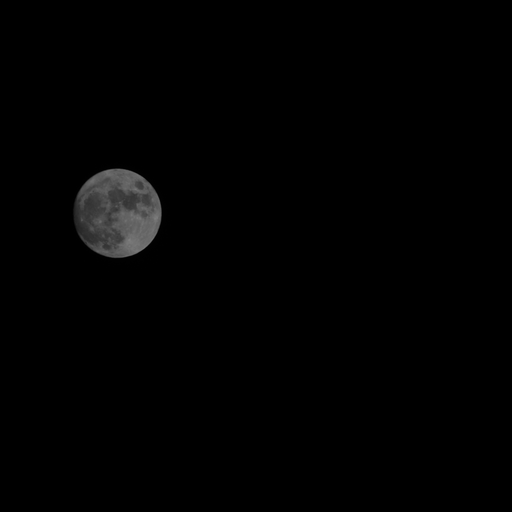
\includegraphics[width=.45\linewidth]{img/best-boss-5162}%
			\label{fig_first_case}}
		\hfil
		\subfloat[]{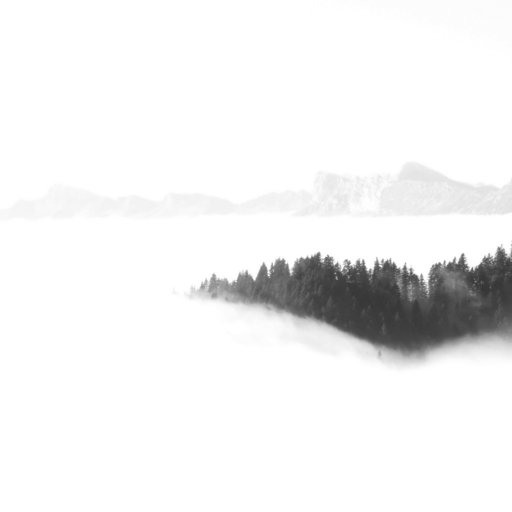
\includegraphics[width=.45\linewidth]{img/best-bows2-1478}%
			\label{fig_second_case}}
		\caption{Images with maximum capacity. (a) BOSSBase/5162.tiff. (b) BOWS2/1478.tiff.}
		\label{fig:best}
	\end{figure}
	
	\begin{figure}[!t]
		\centering
		\subfloat[]{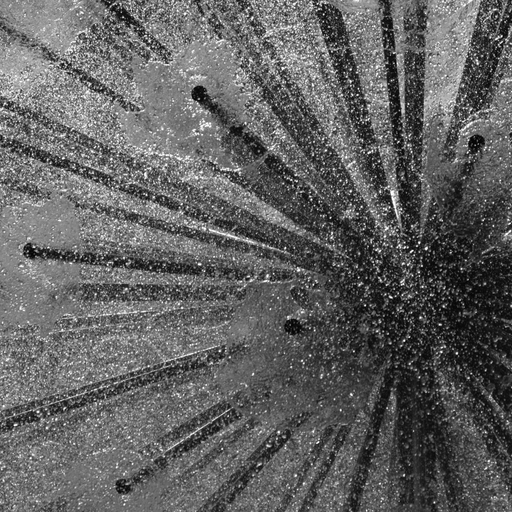
\includegraphics[width=.45\linewidth]{img/worst-boss-1377}%
			\label{fig_first_case2}}
		\hfil
		\subfloat[]{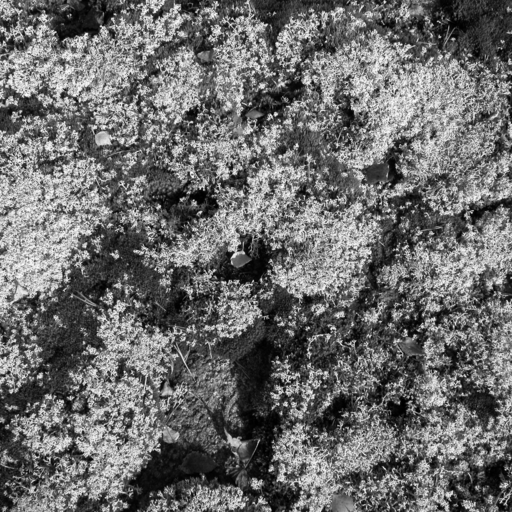
\includegraphics[width=.45\linewidth]{img/worst-bows2-5547}%
			\label{fig_second_case2}}
		\caption{Images with minimum capacity. (a) BOSSBase/1377.tiff. (b) BOWS2/5547.tiff.}
		\label{fig:worst}
	\end{figure}
	
	
	Though our method outperforms the method of other's (as shown in Table~\ref{tab:compare}), it is worths mentioning that, 
	as expected, our method perform better when applied on smooth images since similar adjacent pixels produce larger \(t \in \mathbf{T}\), hence increase the capacity. 
	But with rough images, such as those shown in Fig.\,\ref{fig:worst}, our method produce less satisfactory results.
	
	

%	\section{Conclusion}
\label{sec:conclusion}

In this paper, we analyzed an existed reversible data hiding method proposed by Yin et al., and we proposed three improvements, within which, two of them have significant incremental in embedding capacity that has been shown in Section~\ref{sec:experimental}, while the last improvement aimed to make the method more stable and generalize that can accept cover images of larger size. 

Since the method within our discussion is a reversible data hiding method, 
which can losslessly restore the cover image after extracting secret message, 
and also because the stego image is indeed an encrypted image, 
we omitted the comparison using PSNR and MSE in Section~\ref{sec:experimental} for their value will always be $+\infty$ and $0$.
We focused our comparison on the embedding capacity, i.e., BPP, and the experimental result of applying both method shows that our proposal is superior even in the worst case scenario when applying on rough images. 

\section{Conclusion}
\label{sec:conclusion}

In this paper, 
%we analyzed an existed reversible data hiding method proposed by Yin et al., and 
we proposed a new RDHEI methods that 
%three improvements, within which, two of them 
have significant incremental in embedding capacity.
% that has been shown in Sec.\,\ref{sec:experimental}, while the last improvement aimed to make the method more stable and generalize so that it can accept cover images of larger size. 
Since the method within our discussion is a reversible data hiding method, 
which can losslessly restore the cover image after extracting secret message, 
and also because the stego image is actually an encrypted image, 
we omitted the comparison using PSNR and MSE in Sec.\,\ref{sec:experimental} for their values will always be \(+\infty\) and \(0\).
We focused our comparison on the embedding capacity, i.e., BPP, and the experimental result
% of applying both methods 
 shows that our proposal is superior even in the worst-case scenario when applying on rough images. 
	
	
	
	\subsubsection*{Acknowledgments}
	This research was partially supported by the Ministry of Science and Technology of the Republic of China under the Grants MOST 110-2221-E-015-001-MY3 and MOST 110-2218-E-218-001.
	
	
	\bibliography{shorter_huffman}
	
	%	\appendix
	%	\section{Huffman Coding Tree}

The Huffman coding tree generation process of Lena $512 \times 512$.

\begin{scriptsize}
	\centering
	\begin{longtable}{c}
		\label{app:htree}
		\begin{tabular}{ c  c  c  c  c  c  c  c  c  c } \toprule
			$freq(t)$   &\cellcolor{lightgray} 9818 & \cellcolor{lightgray}9742 & 15247 & 33246 & 44509 & 53359 & 41758 & 24353 & 29089 
			\\ \midrule
			tree
			& \Tree[. [.0 ] ]  
			& \Tree[. [.1 ] ]  
			& \Tree[. [.2 ] ] 
			& \Tree[. [.3 ] ] 
			& \Tree[. [.4 ] ] 
			& \Tree[. [.5 ] ] 
			& \Tree[. [.6 ] ] 
			& \Tree[. [.7 ] ] 
			& \Tree[. [.8 ] ]     
		\end{tabular}
		\\
		\begin{tabular}{ c  c  c  c  c  c  c  c  c } \toprule
			$freq(t)$   &\cellcolor{lightgray} 15247 & 33246 & 44509 & 53359 & 41758 & 24353 & 29089 & \cellcolor{lightgray}19560 
			\\ \midrule
			tree 
			& \Tree[. [.2 ] ]
			& \Tree[. [.3 ] ]
			& \Tree[. [.4 ] ]
			& \Tree[. [.5 ] ]
			& \Tree[. [.6 ] ]
			& \Tree[. [.7 ] ]
			& \Tree[. [.8 ] ]  
			& \Tree[. [.9742 [.1 ]] [.9818 [.0 ] ] ]  
		\end{tabular}
		\\
		\begin{tabular}{ c  c  c  c  c   c  c  c } \toprule
			$freq(t)$  & 33246 & 44509 & 53359 & 41758 & \cellcolor{lightgray}24353 & \cellcolor{lightgray}29089 & 34807 
			\\ \midrule
			tree
			& \Tree[. [.3 ] ]
			& \Tree[. [.4 ] ]
			& \Tree[. [.5 ] ]
			& \Tree[. [.6 ] ]
			& \Tree[. [.7 ] ]
			& \Tree[. [.8 ] ]   
			& \Tree[. [.15247 [.2 ] ] [.19560  [.9742 [.1 ]] [.9818 [.0 ] ] ]]
		\end{tabular}
		\\
		\begin{tabular}{ c   c  c  c   c  c  c } \toprule
			$freq(t)$   & \cellcolor{lightgray}33246   & 44509 & 53359 & 41758 & \cellcolor{lightgray}34807& 53442 
			\\ \midrule
			tree
			& \Tree[. [.3 ] ]
			& \Tree[. [.4 ] ]
			& \Tree[. [.5 ] ]
			& \Tree[. [.6 ] ]
			& \Tree[. [.15247 [.2 ] ] [.19560  [.9742 [.1 ]] [.9818 [.0 ] ] ]]
			& \Tree[. [.24353 [.7 ] ] [.29089 [.8 ] ] ]   
		\end{tabular}
		\\
		\begin{tabular}{  c  c  c   c  c  c } \toprule
			$freq(t)$      & \cellcolor{lightgray}44509 & 53359& \cellcolor{lightgray}41758& 53442& 68053 
			\\ \midrule
			tree
			& \Tree[. [.4 ] ]
			& \Tree[. [.5 ] ]
			& \Tree[. [.6 ] ]
			& \Tree[. [.24353 [.7 ] ] [.29089 [.8 ] ] ]  
			& \Tree[. [.33246 [.3 ] ] [.34807 [.15247 [.2 ] ] [.19560  [.9742 [.1 ]] [.9818 [.0 ] ] ]]] 
		\end{tabular}
		\\
		\begin{tabular}{  c  c   c  c  c } \toprule
			$freq(t)$  & \cellcolor{lightgray}53359& \cellcolor{lightgray}53442& 68053 & 86267 
			\\ \midrule
			tree
			& \Tree[. [.5 ] ]
			& \Tree[. [.24353 [.7 ] ] [.29089 [.8 ] ] ]  
			& \Tree[. [.33246 [.3 ] ] [.34807 [.15247 [.2 ] ] [.19560  [.9742 [.1 ]] [.9818 [.0 ] ] ]]] 
			& \Tree[. [.41758 [.6 ] ] [.44509 [.4 ] ]]
		\end{tabular}
		\\
		\begin{tabular}{  c   c  c  c } \toprule
			$freq(t)$  & \cellcolor{lightgray}68053 & \cellcolor{lightgray}86267& 106801 
			\\ \midrule
			tree
			& \Tree[. [.33246 [.3 ] ] [.34807 [.15247 [.2 ] ] [.19560  [.9742 [.1 ]] [.9818 [.0 ] ] ]]] 
			& \Tree[. [.41758 [.6 ] ] [.44509 [.4 ] ]]
			& \Tree[. [.53359 [.5 ] ] [.53442 [.24353 [.7 ] ] [.29089 [.8 ] ] ] ]
		\end{tabular}
		\\
		\begin{tabular}{ c  c  c } \toprule
			$freq(t)$   & \cellcolor{lightgray}106801& \cellcolor{lightgray}154320 
			\\ \midrule
			tree
			& \Tree[. [.53359 [.5 ] ] [.53442 [.24353 [.7 ] ] [.29089 [.8 ] ] ] ]
			& \Tree[. [.68053 [.33246 [.3 ] ] [.34807 [.15247 [.2 ] ] [.19560  [.9742 [.1 ]] [.9818 [.0 ] ] ]]]  [.86267 [.41758 [.6 ] ] [.44509 [.4 ] ]]]
		\end{tabular}
		\\
		\begin{tabular}{ c  c } \toprule
			$freq(t)$   & \cellcolor{lightgray}261121 
			\\ \midrule
			tree
			& \Tree[. [.106801 [.53359 [.5 ] ] [.53442 [.24353 [.7 ] ] [.29089 [.8 ] ] ] ] [.154320 [.68053 [.33246 [.3 ] ] [.34807 [.15247 [.2 ] ] [.19560  [.9742 [.1 ]] [.9818 [.0 ] ] ]]]  [.86267 [.41758 [.6 ] ] [.44509 [.4 ] ]]]]
			\\ \hline
			code
			& {\Tree[. [.0 [.0 \{00\}\\5 ]
				[.1 [.0 \{010\}\\7 ] [.1 \{011\}\\8 ]]]
				[.1 [.0 [.0 \{100\}\\3 ]
				[.1 [.0 \{1010\}\\2 ]
				[.1 [.0 \{10110\}\\1 ] [.1 \{10111\}\\0 ]]]]
				[.1 [.0 \{110\}\\6 ] [.1 \{111\}\\4 ]]]] }
		\end{tabular}
		\\
	\end{longtable}
\end{scriptsize}
	%	\section{Huffman Tree Serialization}

\subsection{Serialization}


The serialization process of the Huffman tree generated from Lena $512 \times 512$.

\begin{scriptsize}
	\centering
	\begin{longtable}{cc}
		\label{app:serial}
		\begin{tabular}{l}
			\Tree[.$\blacktriangleright\circ\phantom{\blacktriangleright}$ [.$\circ$ 5 
			[.$\circ$ 7  8 ]]
			[.$\circ$ [.$\circ$ 3 
			[.$\circ$  2 
			[.$\circ$  1  0 ]]]
			[.$\circ$  6  4 ]]]
			\\
			\underline{1} \underline{ } \underline{ } \underline{ }
			\underline{ } \underline{ } \underline{ } \underline{ }
			\underline{ } \underline{ } \underline{ } \underline{ }
			\underline{ } \underline{ } \underline{ } \underline{ }
			\underline{ }
			\\
			\underline{ } \underline{ } \underline{ }
			\underline{ } \underline{ } \underline{ }
			\underline{ } \underline{ } \underline{ }
		\end{tabular}
		&
		\begin{tabular}{l}
			\Tree[.$\circ$ [.$\blacktriangleright\circ\phantom{\blacktriangleright}$ 5 
			[.$\circ$ 7  8 ]]
			[.$\circ$ [.$\circ$ 3 
			[.$\circ$  2 
			[.$\circ$  1  0 ]]]
			[.$\circ$  6  4 ]]]
			\\
			\underline{1} \underline{1} \underline{ } \underline{ }
			\underline{ } \underline{ } \underline{ } \underline{ }
			\underline{ } \underline{ } \underline{ } \underline{ }
			\underline{ } \underline{ } \underline{ } \underline{ }
			\underline{ }
			\\
			\underline{ } \underline{ } \underline{ }
			\underline{ } \underline{ } \underline{ }
			\underline{ } \underline{ } \underline{ }
		\end{tabular}
		\\
		\begin{tabular}{l}
			\Tree[.$\circ$ [.$\circ$ {$\blacktriangleright 5 \phantom{\blacktriangleright}$} 
			[.$\circ$ 7  8 ]]
			[.$\circ$ [.$\circ$ 3 
			[.$\circ$  2 
			[.$\circ$  1  0 ]]]
			[.$\circ$  6  4 ]]]
			\\
			\underline{1} \underline{1} \underline{0} \underline{ }
			\underline{ } \underline{ } \underline{ } \underline{ }
			\underline{ } \underline{ } \underline{ } \underline{ }
			\underline{ } \underline{ } \underline{ } \underline{ }
			\underline{ }
			\\
			\underline{0101} \underline{ } \underline{ }
			\underline{ } \underline{ } \underline{ }
			\underline{ } \underline{ } \underline{ }
		\end{tabular}
		&
		\begin{tabular}{l}
			\Tree[.$\circ$ [.$\circ$ 5 
			[.$\blacktriangleright\circ\phantom{\blacktriangleright}$ 7  8 ]]
			[.$\circ$ [.$\circ$ 3 
			[.$\circ$  2 
			[.$\circ$  1  0 ]]]
			[.$\circ$  6  4 ]]]
			\\
			\underline{1} \underline{1} \underline{0} \underline{1}
			\underline{ } \underline{ } \underline{ } \underline{ }
			\underline{ } \underline{ } \underline{ } \underline{ }
			\underline{ } \underline{ } \underline{ } \underline{ }
			\underline{ }
			\\
			\underline{0101} \underline{ } \underline{ }
			\underline{ } \underline{ } \underline{ }
			\underline{ } \underline{ } \underline{ }
		\end{tabular}
		\\
		\begin{tabular}{l}
			\Tree[.$\circ$ [.$\circ$ 5 
			[.$\circ$ {$\blacktriangleright 7 \phantom{\blacktriangleright}$} 8 ]]
			[.$\circ$ [.$\circ$ 3 
			[.$\circ$  2 
			[.$\circ$  1  0 ]]]
			[.$\circ$  6  4 ]]]
			\\
			\underline{1} \underline{1} \underline{0} \underline{1}
			\underline{0} \underline{ } \underline{ } \underline{ }
			\underline{ } \underline{ } \underline{ } \underline{ }
			\underline{ } \underline{ } \underline{ } \underline{ }
			\underline{ }
			\\
			\underline{0101} \underline{0111} \underline{ }
			\underline{ } \underline{ } \underline{ }
			\underline{ } \underline{ } \underline{ }
		\end{tabular}
		&
		\begin{tabular}{l}
			\Tree[.$\circ$ [.$\circ$ 5 
			[.$\circ$ 7 {$\blacktriangleright 8 \phantom{\blacktriangleright}$} ]]
			[.$\circ$ [.$\circ$ 3 
			[.$\circ$  2 
			[.$\circ$  1  0 ]]]
			[.$\circ$  6  4 ]]]
			\\
			\underline{1} \underline{1} \underline{0} \underline{1}
			\underline{0} \underline{0} \underline{ } \underline{ }
			\underline{ } \underline{ } \underline{ } \underline{ }
			\underline{ } \underline{ } \underline{ } \underline{ }
			\underline{ }
			\\
			\underline{0101} \underline{0111} \underline{1000}
			\underline{ } \underline{ } \underline{ }
			\underline{ } \underline{ } \underline{ }
		\end{tabular}
		\\
		\begin{tabular}{l}
			\Tree[.$\circ$ [.$\circ$ 5 
			[.$\circ$ 7 8 ]]
			[.$\blacktriangleright\circ\phantom{\blacktriangleright}$ [.$\circ$ 3 
			[.$\circ$  2 
			[.$\circ$  1  0 ]]]
			[.$\circ$  6  4 ]]]
			\\
			\underline{1} \underline{1} \underline{0} \underline{1}
			\underline{0} \underline{0} \underline{1} \underline{ }
			\underline{ } \underline{ } \underline{ } \underline{ }
			\underline{ } \underline{ } \underline{ } \underline{ }
			\underline{ }
			\\
			\underline{0101} \underline{0111} \underline{1000}
			\underline{ } \underline{ } \underline{ }
			\underline{ } \underline{ } \underline{ }
		\end{tabular}
		&
		\begin{tabular}{l}
			\Tree[.$\circ$ [.$\circ$ 5 
			[.$\circ$ 7 8 ]]
			[.$\circ$ [.$\blacktriangleright\circ\phantom{\blacktriangleright}$ 3 
			[.$\circ$  2 
			[.$\circ$  1  0 ]]]
			[.$\circ$  6  4 ]]]
			\\
			\underline{1} \underline{1} \underline{0} \underline{1}
			\underline{0} \underline{0} \underline{1} \underline{1}
			\underline{ } \underline{ } \underline{ } \underline{ }
			\underline{ } \underline{ } \underline{ } \underline{ }
			\underline{ }
			\\
			\underline{0101} \underline{0111} \underline{1000}
			\underline{ } \underline{ } \underline{ }
			\underline{ } \underline{ } \underline{ }
		\end{tabular}
		\\
		\begin{tabular}{l}
			\Tree[.$\circ$ [.$\circ$ 5 
			[.$\circ$ 7 8 ]]
			[.$\circ$ [.$\circ$ {$\blacktriangleright 3 \phantom{\blacktriangleright}$} 
			[.$\circ$  2 
			[.$\circ$  1  0 ]]]
			[.$\circ$  6  4 ]]]
			\\
			\underline{1} \underline{1} \underline{0} \underline{1}
			\underline{0} \underline{0} \underline{1} \underline{1}
			\underline{0} \underline{ } \underline{ } \underline{ }
			\underline{ } \underline{ } \underline{ } \underline{ }
			\underline{ }
			\\
			\underline{0101} \underline{0111} \underline{1000}
			\underline{0011} \underline{ } \underline{ }
			\underline{ } \underline{ } \underline{ }
		\end{tabular}
		&
		\begin{tabular}{l}
			\Tree[.$\circ$ [.$\circ$ 5 
			[.$\circ$ 7 8 ]]
			[.$\circ$ [.$\circ$ 3 
			[.$\blacktriangleright\circ\phantom{\blacktriangleright}$  2 
			[.$\circ$  1  0 ]]]
			[.$\circ$  6  4 ]]]
			\\
			\underline{1} \underline{1} \underline{0} \underline{1}
			\underline{0} \underline{0} \underline{1} \underline{1}
			\underline{0} \underline{1} \underline{ } \underline{ }
			\underline{ } \underline{ } \underline{ } \underline{ }
			\underline{ }
			\\
			\underline{0101} \underline{0111} \underline{1000}
			\underline{0011} \underline{ } \underline{ }
			\underline{ } \underline{ } \underline{ }
		\end{tabular}
		\\
		\begin{tabular}{l}
			\Tree[.$\circ$ [.$\circ$ 5 
			[.$\circ$ 7 8 ]]
			[.$\circ$ [.$\circ$ 3 
			[.$\circ$  {$\blacktriangleright 2 \phantom{\blacktriangleright}$} 
			[.$\circ$  1  0 ]]]
			[.$\circ$  6  4 ]]]
			\\
			\underline{1} \underline{1} \underline{0} \underline{1}
			\underline{0} \underline{0} \underline{1} \underline{1}
			\underline{0} \underline{1} \underline{0} \underline{ }
			\underline{ } \underline{ } \underline{ } \underline{ }
			\underline{ }
			\\
			\underline{0101} \underline{0111} \underline{1000}
			\underline{0011} \underline{0010} \underline{ }
			\underline{ } \underline{ } \underline{ }
		\end{tabular}
		&
		\begin{tabular}{l}
			\Tree[.$\circ$ [.$\circ$ 5 
			[.$\circ$ 7 8 ]]
			[.$\circ$ [.$\circ$ 3 
			[.$\circ$  2 
			[.$\blacktriangleright\circ\phantom{\blacktriangleright}$  1  0 ]]]
			[.$\circ$  6  4 ]]]
			\\
			\underline{1} \underline{1} \underline{0} \underline{1}
			\underline{0} \underline{0} \underline{1} \underline{1}
			\underline{0} \underline{1} \underline{0} \underline{1}
			\underline{ } \underline{ } \underline{ } \underline{ }
			\underline{ }
			\\
			\underline{0101} \underline{0111} \underline{1000}
			\underline{0011} \underline{0010} \underline{ }
			\underline{ } \underline{ } \underline{ }
		\end{tabular}
		\\
		\begin{tabular}{l}
			\Tree[.$\circ$ [.$\circ$ 5 
			[.$\circ$ 7 8 ]]
			[.$\circ$ [.$\circ$ 3 
			[.$\circ$  2
			[.$\circ$  {$\blacktriangleright 1 \phantom{\blacktriangleright}$} 0 ]]]
			[.$\circ$  6  4 ]]]
			\\
			\underline{1} \underline{1} \underline{0} \underline{1}
			\underline{0} \underline{0} \underline{1} \underline{1}
			\underline{0} \underline{1} \underline{0} \underline{1}
			\underline{0} \underline{ } \underline{ } \underline{ }
			\underline{ }
			\\
			\underline{0101} \underline{0111} \underline{1000}
			\underline{0011} \underline{0010} \underline{0001}
			\underline{ } \underline{ } \underline{ }
		\end{tabular}
		&
		\begin{tabular}{l}
			\Tree[.$\circ$ [.$\circ$ 5 
			[.$\circ$ 7 8 ]]
			[.$\circ$ [.$\circ$ 3 
			[.$\circ$  2
			[.$\circ$  1 {$\blacktriangleright 0 \phantom{\blacktriangleright}$} ]]]
			[.$\circ$  6  4 ]]]
			\\
			\underline{1} \underline{1} \underline{0} \underline{1}
			\underline{0} \underline{0} \underline{1} \underline{1}
			\underline{0} \underline{1} \underline{0} \underline{1}
			\underline{0} \underline{0} \underline{ } \underline{ }
			\underline{ }
			\\
			\underline{0101} \underline{0111} \underline{1000}
			\underline{0011} \underline{0010} \underline{0001}
			\underline{0000} \underline{ } \underline{ }
		\end{tabular}
		\\
		\begin{tabular}{l}
			\Tree[.$\circ$ [.$\circ$ 5 
			[.$\circ$ 7 8 ]]
			[.$\circ$ [.$\circ$ 3 
			[.$\circ$  2 
			[.$\circ$  1  0 ]]]
			[.$\blacktriangleright\circ\phantom{\blacktriangleright}$  6  4 ]]]
			\\
			\underline{1} \underline{1} \underline{0} \underline{1}
			\underline{0} \underline{0} \underline{1} \underline{1}
			\underline{0} \underline{1} \underline{0} \underline{1}
			\underline{0} \underline{0} \underline{1} \underline{ }
			\underline{ }
			\\
			\underline{0101} \underline{0111} \underline{1000}
			\underline{0011} \underline{0010} \underline{0001}
			\underline{0000} \underline{ } \underline{ }
		\end{tabular}
		&
		\begin{tabular}{l}
			\Tree[.$\circ$ [.$\circ$ 5 
			[.$\circ$ 7 8 ]]
			[.$\circ$ [.$\circ$ 3 
			[.$\circ$  2
			[.$\circ$  1 0 ]]]
			[.$\circ$  {$\blacktriangleright 6 \phantom{\blacktriangleright}$}  4 ]]]
			\\
			\underline{1} \underline{1} \underline{0} \underline{1}
			\underline{0} \underline{0} \underline{1} \underline{1}
			\underline{0} \underline{1} \underline{0} \underline{1}
			\underline{0} \underline{0} \underline{1} \underline{0}
			\underline{ }
			\\
			\underline{0101} \underline{0111} \underline{1000}
			\underline{0011} \underline{0010} \underline{0001}
			\underline{0000} \underline{0110} \underline{ }
		\end{tabular}
		\\
		\begin{tabular}{l}
			\Tree[.$\circ$ [.$\circ$ 5 
			[.$\circ$ 7 8 ]]
			[.$\circ$ [.$\circ$ 3 
			[.$\circ$  2
			[.$\circ$  1 0 ]]]
			[.$\circ$  6 {$\blacktriangleright 4 \phantom{\blacktriangleright}$}  ]]]
			\\
			\underline{1} \underline{1} \underline{0} \underline{1}
			\underline{0} \underline{0} \underline{1} \underline{1}
			\underline{0} \underline{1} \underline{0} \underline{1}
			\underline{0} \underline{0} \underline{1} \underline{0}
			\underline{0}
			\\
			\underline{0101} \underline{0111} \underline{1000}
			\underline{0011} \underline{0010} \underline{0001}
			\underline{0000} \underline{0110} \underline{0100}
		\end{tabular}
		& \\
	\end{longtable}
\end{scriptsize}






\subsection{Unserialization}

The unserialization process of the Huffman tree generated from Lena $512 \times 512$.


\begin{scriptsize}
	\centering
	\begin{longtable}{cc}
		\label{app:unserial}
		\begin{tabular}{l}
			\underline{1} {1} {0} {1} {0} {0} {1} {1}
			{0} {1} {0} {1} {0} {0} {1} {0} {0}
			\\
			{0101}{0111}{1000}{0011}{0010}{0001}{0000}{0110}{0100}
			\\
			\Tree[.$\blacktriangleright\circ\phantom{\blacktriangleright}$ \underline{ } \underline{ } ]
		\end{tabular}
		&
		\begin{tabular}{l}
			{1} \underline{1} {0} {1} {0} {0} {1} {1}
			{0} {1} {0} {1} {0} {0} {1} {0} {0}
			\\
			{0101}{0111}{1000}{0011}{0010}{0001}{0000}{0110}{0100}
			\\
			\Tree[.$\circ$ [.$\blacktriangleright\circ\phantom{\blacktriangleright}$ \underline{ } \underline{ } ] \underline{ } ]
		\end{tabular}
		\\
		\begin{tabular}{l}
			{1} {1} \underline{0} {1} {0} {0} {1} {1}
			{0} {1} {0} {1} {0} {0} {1} {0} {0}
			\\
			\underline{0101}{0111}{1000}{0011}{0010}{0001}{0000}{0110}{0100}
			\\
			\Tree[.$\circ$ [.$\circ$ {$\blacktriangleright 5 \phantom{\blacktriangleright}$} \underline{ } ] \underline{ } ]
		\end{tabular}
		&
		\begin{tabular}{l}
			{1} {1} {0} \underline{1} {0} {0} {1} {1}
			{0} {1} {0} {1} {0} {0} {1} {0} {0}
			\\
			\underline{0101}{0111}{1000}{0011}{0010}{0001}{0000}{0110}{0100}
			\\
			\Tree[.$\circ$ [.$\circ$ 5 
			[.$\blacktriangleright\circ\phantom{\blacktriangleright}$ \underline{ } \underline{ } ]] \underline{ } ]
		\end{tabular}
		\\
		\begin{tabular}{l}
			{1} {1} {0} {1} \underline{0} {0} {1} {1}
			{0} {1} {0} {1} {0} {0} {1} {0} {0}
			\\
			{0101}\underline{0111}{1000}{0011}{0010}{0001}{0000}{0110}{0100}
			\\
			\Tree[.$\circ$ [.$\circ$ 5 
			[.$\circ$ {$\blacktriangleright 7 \phantom{\blacktriangleright}$} \underline{ } ]] \underline{ } ]
		\end{tabular}
		&
		\begin{tabular}{l}
			{1} {1} {0} {1} {0} \underline{0} {1} {1}
			{0} {1} {0} {1} {0} {0} {1} {0} {0}
			\\
			{0101}{0111}\underline{1000}{0011}{0010}{0001}{0000}{0110}{0100}
			\\
			\Tree[.$\circ$ [.$\circ$ 5 
			[.$\circ$ 7 {$\blacktriangleright 8 \phantom{\blacktriangleright}$} ]] \underline{ } ]
		\end{tabular}
		\\
		\begin{tabular}{l}
			{1} {1} {0} {1} {0} {0} \underline{1} {1}
			{0} {1} {0} {1} {0} {0} {1} {0} {0}
			\\
			{0101}{0111}\underline{1000}{0011}{0010}{0001}{0000}{0110}{0100}
			\\
			\Tree[.$\circ$ [.$\circ$ 5 
			[.$\circ$ 7 8 ]] 
			[.$\blacktriangleright\circ\phantom{\blacktriangleright}$ \underline{ } \underline{ } ] ] 
		\end{tabular}
		&
		\begin{tabular}{l}
			{1} {1} {0} {1} {0} {0} {1} \underline{1}
			{0} {1} {0} {1} {0} {0} {1} {0} {0}
			\\
			{0101}{0111}\underline{1000}{0011}{0010}{0001}{0000}{0110}{0100}
			\\
			\Tree[.$\circ$ [.$\circ$ 5 
			[.$\circ$ 7 8 ]] 
			[.$\circ$ 
			[.$\blacktriangleright\circ\phantom{\blacktriangleright}$ \underline{ } \underline{ } ] \underline{ } ] ] 
		\end{tabular}
		\\
		\begin{tabular}{l}
			{1} {1} {0} {1} {0} {0} {1} {1}
			\underline{0} {1} {0} {1} {0} {0} {1} {0} {0}
			\\
			{0101}{0111}{1000}\underline{0011}{0010}{0001}{0000}{0110}{0100}
			\\
			\Tree[.$\circ$ [.$\circ$ 5 
			[.$\circ$ 7 8 ]] 
			[.$\circ$ 
			[.$\circ$ {$\blacktriangleright 3 \phantom{\blacktriangleright}$} \underline{ } ] \underline{ } ] ] 
		\end{tabular}
		&
		\begin{tabular}{l}
			{1} {1} {0} {1} {0} {0} {1} {1}
			{0} \underline{1} {0} {1} {0} {0} {1} {0} {0}
			\\
			{0101}{0111}{1000}\underline{0011}{0010}{0001}{0000}{0110}{0100}
			\\
			\Tree[.$\circ$ [.$\circ$ 5 
			[.$\circ$ 7 8 ]] 
			[.$\circ$ 
			[.$\circ$ 3 
			[.$\blacktriangleright\circ\phantom{\blacktriangleright}$ \underline{ } \underline{ } ] ] \underline{ } ] ] 
		\end{tabular}
		\\
		\begin{tabular}{l}
			{1} {1} {0} {1} {0} {0} {1} {1}
			{0} {1} \underline{0} {1} {0} {0} {1} {0} {0}
			\\
			{0101}{0111}{1000}{0011}\underline{0010}{0001}{0000}{0110}{0100}
			\\
			\Tree[.$\circ$ [.$\circ$ 5 
			[.$\circ$ 7 8 ]] 
			[.$\circ$ 
			[.$\circ$ 3 
			[.$\circ$ {$\blacktriangleright 2 \phantom{\blacktriangleright}$} \underline{ } ] ] \underline{ } ] ] 
		\end{tabular}
		&
		\begin{tabular}{l}
			{1} {1} {0} {1} {0} {0} {1} {1}
			{0} {1} {0} \underline{1} {0} {0} {1} {0} {0}
			\\
			{0101}{0111}{1000}{0011}\underline{0010}{0001}{0000}{0110}{0100}
			\\
			\Tree[.$\circ$ [.$\circ$ 5 
			[.$\circ$ 7 8 ]] 
			[.$\circ$ 
			[.$\circ$ 3 
			[.$\circ$ 2 
			[.$\blacktriangleright\circ\phantom{\blacktriangleright}$ \underline{ } \underline{ } ] ] ] \underline{ } ] ] 
		\end{tabular}
		\\
		\begin{tabular}{l}
			{1} {1} {0} {1} {0} {0} {1} {1}
			{0} {1} {0} {1} \underline{0} {0} {1} {0} {0}
			\\
			{0101}{0111}{1000}{0011}{0010}\underline{0001}{0000}{0110}{0100}
			\\
			\Tree[.$\circ$ [.$\circ$ 5 
			[.$\circ$ 7 8 ]] 
			[.$\circ$ 
			[.$\circ$ 3 
			[.$\circ$ 2 
			[.$\circ$ {$\blacktriangleright 1 \phantom{\blacktriangleright}$} \underline{ } ] ] ] \underline{ } ] ] 
		\end{tabular}
		&
		\begin{tabular}{l}
			{1} {1} {0} {1} {0} {0} {1} {1}
			{0} {1} {0} {1} {0} \underline{0} {1} {0} {0}
			\\
			{0101}{0111}{1000}{0011}{0010}{0001}\underline{0000}{0110}{0100}
			\\
			\Tree[.$\circ$ [.$\circ$ 5 
			[.$\circ$ 7 8 ]] 
			[.$\circ$ 
			[.$\circ$ 3 
			[.$\circ$ 2 
			[.$\circ$ 1 {$\blacktriangleright 0 \phantom{\blacktriangleright}$} ] ] ] \underline{ } ] ] 
		\end{tabular}
		\\
		\begin{tabular}{l}
			{1} {1} {0} {1} {0} {0} {1} {1}
			{0} {1} {0} {1} {0} {0} \underline{1} {0} {0}
			\\
			{0101}{0111}{1000}{0011}{0010}{0001}\underline{0000}{0110}{0100}
			\\
			\Tree[.$\circ$ [.$\circ$ 5 
			[.$\circ$ 7 8 ]] 
			[.$\circ$ 
			[.$\circ$ 3 
			[.$\circ$ 2 
			[.$\circ$ 1 0 ] ] ] [.$\blacktriangleright\circ\phantom{\blacktriangleright}$ \underline{ } \underline{ } ] ] ] 
		\end{tabular}
		&
		\begin{tabular}{l}
			{1} {1} {0} {1} {0} {0} {1} {1}
			{0} {1} {0} {1} {0} {0} {1} \underline{0} {0}
			\\
			{0101}{0111}{1000}{0011}{0010}{0001}{0000}\underline{0110}{0100}
			\\
			\Tree[.$\circ$ [.$\circ$ 5 
			[.$\circ$ 7 8 ]] 
			[.$\circ$ 
			[.$\circ$ 3 
			[.$\circ$ 2 
			[.$\circ$ 1 0 ] ] ] 
			[.$\circ$ {$\blacktriangleright 6 \phantom{\blacktriangleright}$} \underline{ } ] ] ] 
		\end{tabular}
		\\
		\begin{tabular}{l}
			{1} {1} {0} {1} {0} {0} {1} {1}
			{0} {1} {0} {1} {0} {0} {1} {0} \underline{0}
			\\
			{0101}{0111}{1000}{0011}{0010}{0001}{0000}{0110}\underline{0100}
			\\
			\Tree[.$\circ$ [.$\circ$ 5 
			[.$\circ$ 7 8 ]] 
			[.$\circ$ 
			[.$\circ$ 3 
			[.$\circ$ 2 
			[.$\circ$ 1 0 ] ] ] 
			[.$\circ$ 6 {$\blacktriangleright 4 \phantom{\blacktriangleright}$} ] ] ] 
		\end{tabular}
		& \\
	\end{longtable}
\end{scriptsize}

	
	\begin{IEEEbiographynophoto}{Li-Chiun Lin}
		received the master's degree in computer science and engineering from the Université Catholique de Louvain, Belgium.
	\end{IEEEbiographynophoto}
	
	\begin{IEEEbiographynophoto}{Cheng-Ta Huang}
		received the Ph.D.~degree in computer science and information engineering from the National Central University, Taiwan, in 2013. 
		He is currently an Assistant Professor of International Bachelor Program in Informatics and Department of Information Management, Yuan Ze University, Taiwan. His research interests include information security and Image processing.
	\end{IEEEbiographynophoto}
	
	\begin{IEEEbiographynophoto}{Shiuh-Jeng WANG}
		received the Ph.D.~degree in electrical engineering from the National Taiwan University, Taiwan. He is currently a Professor of information management, Central Police University, Taiwan. His research interests include information security, evidence ability and forensic analysis.
		
	\end{IEEEbiographynophoto}
	
	
	
	
	
	
	
\end{document}